\chapter{Error Handling}\label{sec:ErrorHandling}
In software development, robust error handling is critical for building maintainable and reliable systems. But strictly speaking, the title of this chapter should be \bdq{Failure Handling} rather than \bdq{Error Handling}, because not every failure is necessarily an error. The difference between \bdq{Failure} and \bdq{Error} is discussed in this chapter.

\bdq{Handling} in this context has two facets, first the reporting of the event and second the response on the event. Both are also discussed here.

In the context of Java programming, Error handling is often reduced to \bdq{Exception Handling} ­– that this is inappropriate in most case is another topic of this chapter.

A proper error handling is crucial for any code, no matter in which type of program it lives – but the definition of \textit{proper} depends significantly on the type of the final product, as it was defined \tqfullvref{sec:TypesOfProducts}. We will discuss this also.

%------------------------------------------------------------------------------

\section{Some Background, some History}\label{sec:ErrorHandlingHistory}
Programmers have to deal with error or failure handling since the first computer was built.

However, the way errors are handled has changed repeatedly over time, yet certain aspects have remained constant.

To demonstrate this, we use a function designed to convert the content of a string into a number. For the sake of simplicity, we allow only integer values in the range of \texttt{-999} to \texttt{+999}. The sign is optional; if it is missing, a positive number is assumed. Leading zeros are permitted. We also assume that the data type for the return value allows only the values from \texttt{-999} to \texttt{+999} – meaning that we have exactly one return value for any valid argument and none for an invalid argument.

The program flowchart for that function is shown on the next page.
\clearpage
\begin{center}
    % dot -Tjpg -y textToNumber.gv > textToNumber.jpg
	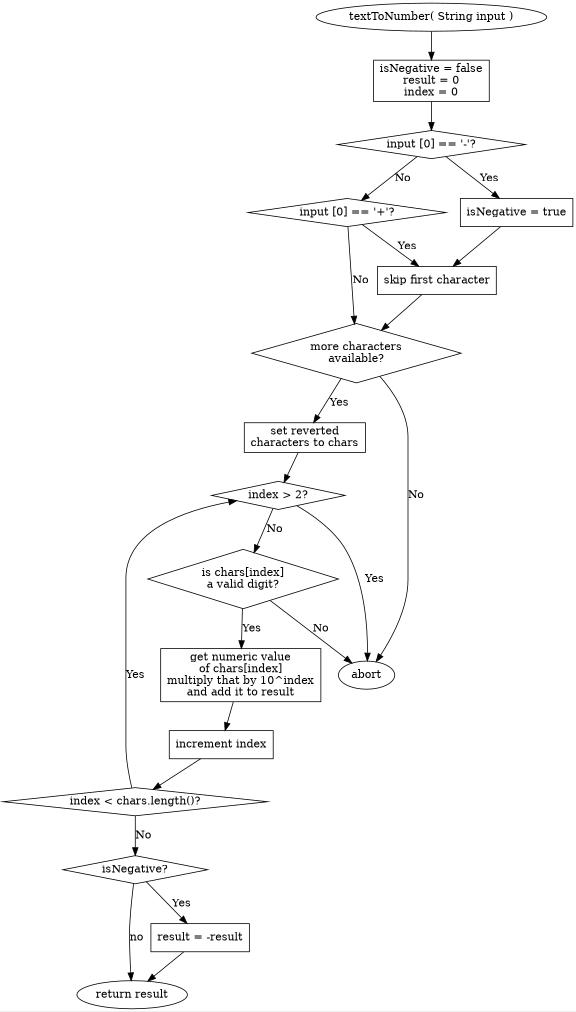
\includegraphics[scale=0.75]{coding/errorHandling/textToNumber}
\end{center}
\clearpage

\keeplisting{16}
The pseudo code for the function would look like this:
\begin{enumerate}[nosep]
	\item{Get the \textit{input} value.}
	\item{If the first character of \textit{input} is \bsq{-}, set the flag \textit{isNegative} to \lstinline|true|, otherwise it is \lstinline|false|.}
    \item{If the first character of \textit{input} is \bsq{+}, skip it.}
    \item{If there are no more characters, abort.}
    \item{Revert the sequence of the remaining characters (\texttt{+123} gets \texttt{321}).}
    \item{Set the \textit{result} to \texttt{0}.}
    \item{Set the \textit{index} to \texttt{0}.}
    \item{If \textit{index} is greater than \texttt{2}, abort.}
    \item{If character on the location determined by \texttt{index} is not a valid digit (something between \texttt{0} and \texttt{9}), abort.}
    \item{Get the numeric value of the character on the location determined by the \textit{index} and multiply that by \texttt{10}\textsuperscript{\textit{index}}.}
    \item{Add that to the \textit{result}.}
    \item{Increment \textit{index}.}
    \item{If \textit{index} is not greater than the number of characters, go back to step~8.}
    \item{If \textit{isNegative} is \lstinline|true|, multiply \textit{result} by \texttt{-1}.}
    \item{Return \textit{result}.}
\end{enumerate}

\keeplisting{23}
We can write this in Java like this:
\begin{lstlisting}
public final int textToNumber( final String input )
{
    var pos = 0;
    var isNegative = false;
    if( input.charAt( pos ) == '-' )
    {
        isNegative = true;
        ++pos;
    }
    else
    {
        if( input.charAt( pos ) == '+' ) ++pos;
    }
    if( pos >= input.length() ) System.exit( -1 );
    final var s = reversed( input.substring( pos ).toCharArray() );
    var result = 0;
    var index = 0;
    while( index < s.length )
    {
        if( index > 2 ) System.exit( -1 );
        if( s [index] < '0' || s [index] > '9' ) System.exit( -1 );
        result += (s [index] - '0') * Math.powExact( 10, index );
        ++index;
    }
    if( isNegative ) result *= -1;
    return result;
}   //  textToNumber()
\end{lstlisting}
Our translation of \bdq{abort} into a call to \lstinline|System.exit()|\index{java.lang!System!exit()} makes the function mostly unusable: it is not really feasible to terminate the current program just because of an invalid input to a data conversion function.

In a language like C\index{C}, we could solve the issue like this:\footnote{Obviously, this is not valid C\index{C} code, but the signature fits the problem.}
\keeplisting{25}
\begin{lstlisting}[language=C]
bool textToNumber( const char* input, int& result )
{
    var pos = 0;
    var isNegative = false;
    if( charAt( input, pos ) == '-' )
    {
        isNegative = true;
        ++pos;
    }
    else
    {
        if( charAt( input, pos ) == '+' ) ++pos;
    }
    if( pos >= length( input ) ) return false; // failed
    var s = reversed( toCharArray( substring( input, pos ) );

    result = 0;
    var index = 0;
    while( index < length( s ) )
    {
        if( index > 2 ) return false; // failed
        if( s [index] < '0' || s [index] > '9' ) return false; // failed
        result += (s [index] - '0') * pow ( 10, index );
        ++index;
    }
    if( isNegative ) result *= -1;

    return true;
}   //  textToNumber()
\end{lstlisting}

You call this method like this:
\begin{lstlisting}[language=C]
int result;
if( !textToNumber( input, result ) )
{
    // Handle the failure;
}
\end{lstlisting}

The fact that the function's return value must be specified as an argument is not particularly intuitive, but there is no other way to handle it, because none of the possible result values can be co-opted to signal an error.\footnote{You can achieve this also in Java, but it would be even more unintuitive than the C\index{C} version.}

\keeplisting{27}
The Go\index{go} programming language solves this problem by allowing a function to have two return values\footnote{Same as above, this is not valid go\index{go} code, by the signature demonstrates how it would work.}:
\begin{lstlisting}[language=go]
func textToNumber(input string) (bool, int)
{
    var pos = 0;
    var isNegative = false;
    if charAt( input, pos ) == '-' {
        isNegative = true;
        ++pos;
    }
    else
    {
        if charAt( input, pos ) == '+' {++pos}
    }
    if pos >= length( input ) { return false, 0 } // failed
    var s = reversed( toCharArray( substring( input, pos ) );

    result = 0;
    var index = 0;
    while( index < length( s ) )
    {
        if index > 2 { return false, 0 } // failed
        if s [index] < '0' || s [index] > '9' { return false, 0 } // failed
        result += (s [index] - '0') * pow 10, index );
        ++index;
    }
    if isNegative { result *= -1}

    return true, result;
}   //  textToNumber()
\end{lstlisting}

\keeplisting{4}
This is called like this:
\begin{lstlisting}[language=go]
ok, result := textToNumber( input );
if !ok {
    // Handle the failure;
}
\end{lstlisting}

In both cases, we now have a status that tells us whether the function was successful or not – so the reporting aspect is resolved.

If we can be certain that the function call will succeed, we do not need to check the status. However, that would require us to validate the function arguments accordingly, which would merely shift the problem: namely, how do we respond to a failure?

The seemingly simple answer is we jump to an error handler, which then terminates the program. Or, if we are inside a function, we simply return an error status ...

C\index{C} allows us to use \lstinline|goto|, and in go\index{go}, even the standard libraries use \lstinline|goto| to jump to a centralized housekeeping section. However, we must check the returned status for every single method call, which does not necessarily make the code more readable. If the actual return value also needs to be checked – and the execution flow might change as a result – the code quickly becomes completely convoluted.

Not to mention that for both C\index{C} and go\index{go}, the \lstinline|goto| allows us to jump only to a label inside the current function, but not to a global error handler.

\keeplisting{28}
To avoid this problem, Java uses exceptions\index{exception} to report failures.\footnote{Java is not the only language that uses exceptions\index{exception}, and it was not the first. But is seen as the first that introduced \lstinline|finally|.} A more sensible Java version of our function would therefore look like this:
\begin{lstlisting}
public final int textToNumber( final String input )
{
    var pos = 0;
    var isNegative = false;
    if( input.charAt( pos ) == '-' )
    {
        isNegative = true;
        ++pos;
    }
    else
    {
        if( input.charAt( pos ) == '+' ) ++pos;
    }
    if( pos >= input.length() ) throw new RuntimeException( "No more characters" );
    final var s = reversed( input.substring( pos ).toCharArray() );

    var result = 0;
    var index = 0;
    while( index < s.length )
    {
        if( index > 2 ) throw new RuntimeException( "Too many digits" );
        if( s [index] < '0' || s [index] > '9' )  throw new RuntimeException( "Invalid character: " + s [index] );
        result += (s [index] - '0') * Math.powExact( 10, index );
        ++index;
    }
    if( isNegative ) result *= -1;

    return result;
}   //  textToNumber()
\end{lstlisting}

Chapter \tqfullvref{sec:ErrorsAndExceptions} provides more insight into exceptions\index{exception} in Java. 

\keeplisting{8}
If you want to deal with the failure, you will call \lstinline|textToNumber()| like this:
\begin{lstlisting}
try
{
    final var number = textToNumber( text );
}
catch( final RuntimeException e )
{
    // Handle the exception
}
\end{lstlisting}

If we want to delegate that failure to a higher level, we just call \lstinline|textToNumber()|, and ignore the exception\index{exception}; it \textit{bubbles up} automatically:
\begin{lstlisting}
final var number = textToNumber( text );
\end{lstlisting}

Looks like the perfect solution to our problem. Unfortunately, there is nothing like a free lunch, as we will see in the \hyperref[sec:ExceptionCosts]{next} chapter.

%==============================================================================
% End of file!!
%==============================================================================

\section{The Costs of Throwing an Exception}\label{sec:ExceptionCosts}
To understand this section, some background knowledge regarding the interaction between the Java compiler \texttt{javac}\index{javac}, the \Java Virtual Machine (JVM), and the integrated JIT\index{JIT} compiler (HotSpot\index{HotSpot} for Oracle's JVM) is helpful.

The Java compiler \texttt{javac}\index{javac} translates Java source code into Java bytecode ­– a form of \bdq{machine language} executed interpretively within a virtual machine (the JVM) ­– entailing the performance issues inherent to interpreters.

As mentioned, the JIT\index{JIT} (just-in-time) compiler is a component of the JVM; it translates Java bytecode into native machine code at runtime, while the program is executed. However, only code that is executed repeatedly is translated; furthermore, the generated machine code may be discarded and replaced with newly generated code as part of further optimizations.

This mechanism is responsible for the steady increase in a Java program's throughput over time until a saturation point is reached.

It should be equally obvious that throughput collapses when the JVM must discard the generated machine code and revert to executing the Java bytecode in interpreter mode.

%------------------------------------------------------------------------------

\subsection{What happens when an Exception is thrown?}
\begin{enumerate}
	\item{Object Creation and Stack Trace Capture
	 
	When \bdq{\lstinline|throw new FooException()|} is executed, normal object allocation happens, then the constructor\index{constructor} of \lstinline|java.lang.Throwable|\index{java.lang!Throwable} \autocite{ORACLE_DOC_THROWABLE_CLASS} calls the native method \lstinline|fillInStackTrace()|\index{java.lang!Throwable!fillInStackTrace()} \autocite{ORACLE_DOC_THROWABLE:fillInStackTrace}. This runs synchronously in the throwing thread itself (no safepoint is needed, since it is inspecting its own stack) and builds a compact internal backtrace structure – not yet the finished \lstinline|StackTraceElement[]|\index{java.lang!StackTraceElement} array \autocite{ORACLE_DOC_STACKTRACEELEMENT_CLASS}. That array only materializes lazily when \lstinline|Throwable::getStackTrace|\index{java.lang!Throwable!getStackTrace()} \autocite{ORACLE_DOC_THROWABLE:getStackTrace} or \lstinline|Throwable::printStackTrace|\index{java.lang!Throwable!printStackTrace()} \autocite{ORACLE_DOC_THROWABLE:printStackTrace} is called.
	
	For the JVM-internal exceptions
	\begin{itemize}[nosep]
		\item{\lstinline|java.lang.ArithmeticException|\index{java.lang!ArithmeticException} \autocite{ORACLE_DOC_ARITHMETICEXCEPTION_CLASS}}
		\item{\lstinline|java.lang.ArrayIndexOutOfBoundsException|\index{java.lang!ArrayIndexOutOfBoundException} \autocite{ORACLE_DOC_ARRAYINDEXOUTOFBOUNDSEXCEPTION_CLASS}}
		\item{\lstinline|java.lang.ArrayStoreException|\index{java.lang!ArrayStoreException} \autocite{ORACLE_DOC_ARRAYSTOREEXCEPTION_CLASS}}
		\item{\lstinline|java.lang.ClassCastException|\index{java.lang!ClassCastException} \autocite{ORACLE_DOC_CLASSCASTEXCEPTION_CLASS}}
		\item{\lstinline|java.lang.NullPointerException|\index{java.lang!NullPointerException} \autocite{ORACLE_DOC_NULLPOINTEREXCEPTION_CLASS}}
	\end{itemize}
	there is a specific \bdq{optimization} JVM parameter that is on by default:
	\begin{center}
		\texttt{\mbox{-XX:+OmitStackTraceInFastThrow}}\index{OmitStackTraceInFastThrow}  
	\end{center}
	If the same implicit exception\index{exception} is thrown repeatedly (\bdq{hot}) at the same bytecode location, HotSpot\index{HotSpot} replaces the allocation and the stack-trace-fill step with a preallocated, stack-trace-less instance (\bdq{\texttt{… <no stack trace available>}}). This is the classic reason exceptions\index{exception} used as control flow in loops eventually show up with no stack trace at all – and it is also why \lstinline|NullPointerException|'s\index{java.lang!NullPointerException} helpful detailed messages disappear once this kicks in, since the backtrace data the message relies on is missing.
	
Benchmarks show a call to \lstinline|new Exception()|\index{java.lang!Exception} to instantiate an exception\index{exception} object costs roughly 1200ns versus around 8ns for a simple object like \lstinline|java.util.Date|\index{java.util!Date} (and \lstinline|Date| is far from being really simple).
	
The calls to \lstinline|Throwable::fillInStackTrace|\index{java.lang!Throwable!fillInStackTrace()} causes a measurable CPU load under a high exception rate (e.g., when validation exceptions\index{validation exception}\index{exception} are used to control the execution flow). In addition, the costs for filling the stack trace scales with stack depth that is often in the range of \mbox{50+} frames for code executed within an application server or web container. Of course this affects also the next step.}
	
	\item{\lstinline|athrow|\index{athrow} and Stack Unwinding 
	
	The \lstinline|athrow|\index{athrow} bytecode instruction pops the reference from the stack and starts the handler\footnote{In source code, that \bdq{handler} is a \bsq{\lstinline|catch( final <Exception> e )|}\index{try!catch} line in most cases, where \texttt{<Exception>} matches the type of the thrown exception\index{exception}, or a parent class.} search: the JVM (interpreter or compiled code, via the method's exception table/OopMaps\index{OopMaps}) checks whether the current frame has a matching handler for the thrown exception\index{exception}. The type check is handled via the exception’s\index{exception} class hierarchy.
	
	If no match could be found, the frame is popped from the stack, during which:
	\begin{itemize}
		\item{\lstinline|monitorexit|\index{monitorexit} (another bytecode instruction) runs for every active synchronized\index{synchronized} block/method\index{method!synchronized} in that frame, to release the locks}
		\item{Local variables become eligible for the garbage collection}
		\item{The search continues recursively in the caller frame}
	\end{itemize}
	If no matching handler exists anywhere on the stack, the internal method \lstinline|Thread::dispatchUncaughtException|\index{java.lang!Thread!dispatchUncaughtException()} will call the implementation of the interface \lstinline|UncaughtExceptionHandler|\index{java.lang!Thread.UncaughtExceptionHandler} \autocite{ORACLE_DOC_UNCAUGHTEXCEPTIONHANDLER_INTERFACE} that is either set to the \lstinline|Thread|\index{java.lang!Thread} \autocite{ORACLE_DOC_THREAD_CLASS} object itself or to the associated \lstinline|ThreadGroup|\index{java.lang!ThreadGroup} \autocite{ORACLE_DOC_THREADGROUP_CLASS}. If none is set, the parent thread is searched for an \lstinline|UncaughtExceptionHandler|\index{java.lang!Thread.UncaughtExceptionHandler}.
	Details about \lstinline|UncaughtExceptionHandler|\index{java.lang!Thread.UncaughtExceptionHandler} are provided in chapter \tqfullvref{sec:ExceptionHandlingInThreads}.}
\end{enumerate}

%------------------------------------------------------------------------------

\subsection{JIT Deoptimization}\label{sec:JITDeopt}
This is where the real cost lies if things go wrong.
 
The JIT\index{JIT} compiler profiles exception paths. If a \lstinline|catch|\index{try!catch} branch is rarely or never taken during profiling, the compiler often doesn't compile it in fully – it places an \textit{uncommon} trap there instead. If that path is then actually hit at runtime, it triggers a \textit{deoptimization of that specific method}\index{method}: execution falls back to the interpreter for that frame and continues interpreted from there.

\bdq{Deoptimization} means the compiler's optimistic assumption was proven wrong, so execution switches from compiled code back to the interpreter by reconstructing interpreter state, and the compiled code may either be discarded or recompiled.

Whether the affected method\index{method} gets recompiled depends on the trap history (\texttt{PerMethodTrapLimit}/\texttt{PerBytecodeTrapLimit}). If the trap fires too often, HotSpot\index{HotSpot} permanently marks the method as no longer compilable for that path at full optimization – it stays interpreted or degraded.

Simply throwing/catching exceptions through code that was already compiled with the handler correctly baked in from the start does \textit{not} cause deoptimization – unwinding through compiled frames runs through generated runtime stubs, GC-safe via OopMaps, without falling back to the interpreter.

In short: deoptimization doesn't happen because of the \lstinline|throw| itself, but when the exception\index{exception} activates an execution path the compiler had classified as \bdq{cold} at compile time.

Practical takeaway: exceptions\index{exception} for genuine error cases (rare, truly exceptional) are essentially free in practice. Exceptions\index{exception} used as regular control flow (e.g., validation on every request) are the case where stack trace cost, garbage collection pressure, and deoptimization churn actually matter – there it's often worth avoiding exceptions\index{exception} as a signaling mechanism.

%==============================================================================
% End of file!!
%==============================================================================


\section{Not every Failure is an Error}\label{sec:FailureVsError}
As said above: using exceptions\index{exception} for real errors does not harm, but for mere failures, they are far from being the silver bullet.

But when is a failure an error?

Let’s go back to the \lstinline|textToNumber()| method which we have already cited above. The need to convert a string consisting solely of digits into the numerical value it represents may arise at various points in a program; below some sample scenarios:
\begin{enumerate}[label=Scenario \arabic*:,leftmargin=8em]
	\item{Parsing the command line arguments during program startup}
	\item{Reading a configuration parameter from a configuration file, again during startup}
	\item{Parsing the arguments of an HTTP request}
	\item{Interpreting the incoming data on a REST response}
	\item{Handling the user input from a UI}
	\item{Reading data that was previously stored by the same program}
\end{enumerate}

Obviously, our response on a failure of \lstinline|textToNumber()| should be different depending on the use case.

In the first and perhaps even the second scenario, the program would need to abort if the conversion from text to a number fails. Here that failure is clearly an error. For these cases, one could even use the very first version of the \lstinline|textToNumber()| method (that one calling \lstinline|System.exit()|\index{java.lang!System!exit()} upon failure). The second scenario may define a default value that is used in case the conversion of the configuration value failed, avoiding the program abort.

Perhaps aborting the program would be even the proper behaviour in scenario~6, although it is more likely that you would abandon the current record, somehow report the failure to the user and proceed with the next record.

But for scenarios~3, 4 and 5, our program gets invalid data from an external source. So, it should reflect that to that source (by sending a \texttt{\mbox{5xx}} status code or returning an error code to the requestor in case of 3 and 4, or by displaying a window with an error message in scenario~5). These cases are not errors, at least not from our point of view.

Of course, we want to have only one implementation of \lstinline|textToNumber()| that fits all scenarios. That eliminates obviously the very first implementation attempt. But based on what we know from the \hyperref[sec:ExceptionCosts]{previous} chapter, it is not acceptable to use exceptions\index{exception} for the flow control, due to their potential costs. That means that we cannot use the last version of our function, too, at least not for the scenarios~3, 4, and 5.

The cost for the exceptions\index{exception} does not matter for the scenarios~1 and 2, because the program aborts afterwards, and it can be ignored for scenario~6, because \lstinline|textToNumber()| normally does not fail in this case.

But for the remaining three scenarios, we may have to face a lot of failures and should therefore avoid the use of exceptions. Luckily, this requirement is not new, and the problem with the special values for reporting a failure is well known. The answer for that is coming with the classes
\begin{itemize}[nosep]
	\item{\lstinline|java.util.Optional<T>|\index{java.util!Optional} \autocite{ORACLE_DOC_OPTIONAL_CLASS}}
	\item{\lstinline|java.util.OptionalDouble|\index{java.util!OptionalDouble} \autocite{ORACLE_DOC_OPTIONALDOUBLE_CLASS}}
	\item{\lstinline|java.util.OptionalInt|\index{java.util!OptionalInt} \autocite{ORACLE_DOC_OPTIONALINT_CLASS}}
	\item{\lstinline|java.util.OptionalLong|\index{java.util!OptionaLong} \autocite{ORACLE_DOC_OPTIONALLONG_CLASS}}
\end{itemize}

For our use case, \lstinline|OptionalInt|\index{java.util!OptionalInt} is the proper tool.

\keeplisting{35}
Here is an implementation of \lstinline|textToNumber()| that uses \lstinline|OptionalInt|\index{java.util!OptionalInt} as the return value: 
\begin{lstlisting}
public final OptionalInt textToNumber( final String input )
{
    if( isNull( input ) ) throw new IllegalArgumentException( "input is null" );
    OptionalInt retValue = OptionalInt.empty();
    var pos = 0;
    var isNegative = false;
    if( input.charAt( pos ) == '-' )
    {
        isNegative = true;
        ++pos;
    }
    else
    {
        if( input.charAt( pos ) == '+' ) ++pos;
    }
    if( pos < input.length() )
    {
        final var s = reversed( input.substring( pos ).toCharArray() );

        var result = 0;
        var index = 0;
        SumLoop: while( index < s.length )
        {
            if( index > 2 || s [index] < '0' || s [index] > '9' )
            {
                index = -1;
                break SumLoop;
            }
            result += (s [index] - '0') * Math.powExact( 10, index );
            ++index;
        }   //  SumLoop:
        if( index > 0 )
        {
            if( isNegative ) result *= -1;
            retValue = OptionalInt.of( result );
        }
    }

    return retValue;
}   //  textToNumber()
\end{lstlisting}

\keeplisting{2}
Generally, \lstinline|textToNumber()| can be called like this now:
\index{java.util!OptionalInt!ifPresentOrElse()}
\begin{lstlisting}
textToNumber( input ).ifPresentOrElse( IO::println, () -> println( "Invalid Input" );
\end{lstlisting}

\keeplisting{6}
For scenario~1, the call may look like this:
\index{java.util!OptionalInt!isEmpty()}
\begin{lstlisting}
final var result = textToNumber( input );
if( result.isEmpty() )
{
    err.printf( "Invalid Number on command line: %s%nProgram aborted!%n", input );
    System.exit( -1 );
}
\end{lstlisting}

\keeplisting{6}
For scenario~2, it would be more or less the same than for scenario~1, only the message written to the console may differ. But when there is a default value that can be used in case of a missing or invalid configuration value, the call can look like this:
\index{java.util!OptionalInt!orElse()}
\begin{lstlisting}
final var configValue = textToNumber( input ).orElse( 42 );
\end{lstlisting}

For scenario~3, our program implemented \lstinline|HttpServlet::doGet|\index{jakarta.servlet.http!HttpServlet!goGet()} \autocite{JAKARTA_EE_HTTPSERVLET_CLASS,JAKARTA_EE_HTTPSERVLET::doGet} that processes the incoming HTTP\index{HTTP} requests. It parses the request parameters and aborts in case of a failure:\footnote{For the sake of the argument, we ignore that there is a method named \lstinline|HttpServletRequest::getIntHeader|\index{jakarta.servlet.http!HttpServletRequest!getIntHeader()} \autocite{JAKARTA_EE_HTTPSERVLETREQUEST_CLASS,JAKARTA_EE_HTTPSERVLETREQUEST::getHeader,JAKARTA_EE_HTTPSERVLETREQUEST::getIntHeader} that returns the integer value of the request header directly.}
\index{jakarta.servlet.http!HttpServletRequest!getHeader()}
\index{jakarta.servlet.http!HttpServletRequest}
\index{jakarta.servlet.http!HttpServletResponse!sendError()}
\index{jakarta.servlet.http!HttpServletResponse}
\begin{lstlisting}
protected final void doGet( final HttpServletRequest request, final HttpServletResponse response )
{
    final var input = request.getHeader( "INPUT" );
    if( isNull( input ) )
    {
        response.sendError( 555, "No value for INPUT provided" );
        return;
    }
    final var result = textToNumber( input );
    if( result.isEmpty() ) 
    {
        response.sendError( 555, "Value for INPUT is invalid: %s".formatted( input ) );
        return;
    }
}   //  doGet()
\end{lstlisting}
We must check whether \lstinline|input| is not \lstinline|null| before calling \lstinline|textToNumber()| because the method would throw an \lstinline|IllegalArgumentException|\index{java.lang!IllegalArgumentException} \autocite{ORACLE_DOC_ILLEGALARGUMENTEXCEPTION_CLASS} if called with \lstinline|null| as the argument. Of course we could have implemented \lstinline|textToNumber()| to return \lstinline|OptionalInt.empty()|\index{java.util!OptionalInt!empty()} \autocite{ORACLE_DOC_OPTIONALINT:empty} in case of \lstinline|input == null|, but then we could not distinguish the root cause for the failure.

The code for scenario~4 will look similar, just the classes and methods are different; we also have a method that handles the incoming data (here a REST\index{REST} message), and that needs to abort in case the conversion from text to number fails.

\keeplisting{16}
For scenario~5, we have a loop of some kind; it repeats asking the user for a valid number until it gets one. A real UI would allow the user to terminate the current screen alternatively.
\begin{lstlisting}
var repeat = true; 
OptionalInt result;
while( repeat )
{
    final var inputData = ui.retrieveInputData();
    final var input = inputData.get( "input" ); // Will never return null!!
    result = textToNumber( input );
    if( result.isPresent() ) 
    {
        repeat = false;
    }
    else
    { 
        ui.displayMessage( "input", "%s is not a valid number".formatted( input ) );
    }
}
\end{lstlisting}

\keeplisting{20}
The loop for scenario~6 is a little different. Each cycle reads a record and tries to translate the text to a number. If this fails, that record will be discarded, otherwise it is further processed.
\begin{lstlisting}
while( records.hasMore() )
{
    final var dataRecord = records.next();
    final int number;
    try
    {
        number = textToNumber( dataRecord.getInput() ).orElseThrow(); 
    }
    catch( final NoSuchElementException _ )
    {
        reportError( dataRecord, "input", "Not a number" );
        continue;
    }
    catch( final IllegalArgumentException _ )
    {
        reportError( dataRecord, "input", "No value" );
        continue;
    }
    process();
}
\end{lstlisting}

We see that it is possible to avoid exceptions\index{exception} with this last implementation of \lstinline|textToNumber()| in those cases where failures are not errors. We have seen also that we use exceptions\index{exception} only when the failure is not anticipated (meaning where the failure is really exceptional).

Our \lstinline|textToNumber()| method was used only to illustrate how to report failure to the caller; in a real program, you would use \lstinline|Integer::parseInt|\index{java.lang!Integer!parseInt()} \autocite{ORACLE_DOC_INTEGER:parseInt} for the same purpose. The Javadoc documentation for that method says:
\begin{center}
	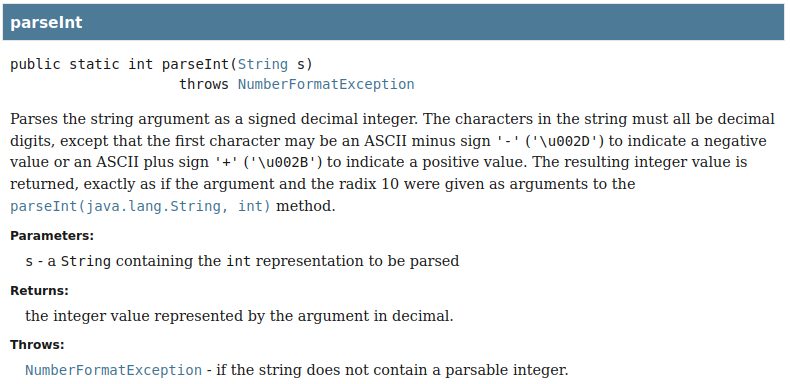
\includegraphics[scale=0.55]{coding/errorHandling/Javadoc_Integer_parseInt}
\end{center}

Obviously, \lstinline|Integer::parseInt|\index{java.lang!Integer!parseInt()} always throws an exception\index{exception} when it cannot parse the given string to a valid integer. This is quite problematic when erroneous input data occurs very frequently, for the reasons described in \tqfullref{sec:ExceptionCosts}.

One solution would be to create your own parser, but the better one is to remember a best practice from the past: validate the input data before you call something with that data as an argument.

\keeplisting{6}
This may look like this:
\begin{lstlisting}
var isValid = nonNull( input ) && !input.isBlank();
if( isValid )
{
    var pos = 0;
    final var len = input.length();
    if( !Character.isDigit( input.charAt( pos ) ) )
    {
        ++pos;
        isValid = input.startsWith( "-" ) || input.startsWith( "+" );
    }(|\clearpage|)    
    while( isValid && pos < len )
    {
        isValid = Character.isDigit( input.charAt( pos++ ) );
    }
}
final OptionalInt result = isValid
    ? OptionalInt.of( Integer.parseInt( input ) )
    : OptionalInt.empty();
\end{lstlisting}

This can be applied to other situations as well. Just assume you want to read some arbitrary files from the filesystem; obviously this fails if the given file name denotes a directory instead of a plain file, or if the necessary permissions to read that file are missing, or if there is no file with the given name. 

The plain simple implementation would be like this:
\keeplisting{6}
\begin{lstlisting}
try
{
    final var contents = Files.readAllLines( Path.of( fileName ) );
}
catch( final InvalidPathException | IOException e )
{
    reportFailure( "Cannot read file %s".formatted( fileName ), e );
}
\end{lstlisting}

Just try it and let it throw an exception\index{exception} in case the file cannot be read. This approach is quite acceptable when it works nearly all the time. If not, you have too many exceptions.

\keeplisting{16}
So better validate the input data before using it:
\begin{lstlisting}
if( isNull( fileName ) ) reportFailure( "filename is null" );
try
{
    final var path = Path.of( fileName );
    if( !Files.exists( path ) )
    {
        reportFailure( "File %s does not exist".formatted( fileName ) );
    }
    else if( !Files.isRegularFile( path ) )
    {
        reportFailure( "File %s is not a regular file".formatted( fileName ) );
    }
    else if( !Files.isReadable( path ) )
    {
        reportFailure( "Cannot read file %s".formatted( fileName ) );
    }(|\clearpage|)
    else
    {
        final var contents = Files.readAllLines( path );
    }
}
catch( final InvalidPathException e )
{
    reportFailure( "Invalid Path: %s".formatted( fileName ), e );
}
catch( final IOException e )
{
    reportFailure( "Unexpected failure reading file %s".formatted( fileName ), e );
}
\end{lstlisting}

We must keep the \lstinline|catch|\index{try!catch} clauses for the \lstinline|IOException|\index{java.io!IOException} and the \lstinline|InvalidPathException|\index{java.nio.file!InvalidPathException} because reading a file can still fail one or the other way, even after we pre-checked and eliminated most of the possible root causes upfront.

Another example for this approach is one that everybody who starts learning programming is taught with one of the first lessons: it is to check whether a numerical value that should be used as a divisor is not zero, before executing the division.

We have seen now that it is possible to avoid exceptions in case of failures that are not necessarily also errors.

But when is a failure an error?

Based on what said above, I suggest the following definition: \bdq{\textit{An Error is a Failure that requires to abort the current operation}}.

It should be obvious that already for technical reasons throwing an exception\index{exception} does always indicate an Error at the level of the current operation. Consequently, catching an exception\index{exception} means that the calling operation will try to fix the error that caused the aborted operation to fail – degrading the Error to a mere Failure.\footnote{But we will see later that it makes sense to catch an exception\index{exception} even when the error condition cannot be fixed.}

%==============================================================================
% End of file!!
%==============================================================================


\section{Reporting Failures and Errors}\label{sec:ReportFailure}
An Error may not remain unnoticed, and to some extent, even Failures should be brought to the attention of the users or administrators of our program.

Usually the reporting of an Error is delegated by the aborted operation to its parent operation (in case of a method\index{method} call, the aborted method\index{method} relayed it to the method\index{method} that called it). But at some level, there isn’t a parent operation anymore – so how to report at this level?

\subsection{Ways to Report}
Basically, these are ways an operation (a method\index{method}) has to externalise an error condition (to bring it to the attention of the users or administrators):

\paragraph{Return a status as the return value of the method\index{method} call} – We discussed this already \hyperref[sec:FailureVsError]{above}. It requires that the calling method\index{method} checks the return value to detect the failure, but it does not externalises the error condition. This remains the task of the caller. 

\paragraph{Set a global status flag} – This approach can cause issues in multithreaded environments, because it may be difficult to synchronize concurrent updates to the global field that represents the status flag.

It also requires the calling method\index{method} to check that flag after each call, and it also leaves the externalisation of the error condition to the caller.

You should always prefer a return value for the status over a global status flag, and if that is not feasible, throwing an exception\index{exception} still might be the better option.

\paragraph{Write a message to the console} – This immediately externalises the error condition, but in the most volatile way. Nevertheless, depending on the context, this may be sufficient.

\paragraph{Open a message window} – Obviously this make sense only for an application with some kind of UI. Usually, such a message window (or \bdq{Message Box}) provides options on how to proceed.

This is similarly volatile as writing the message to the console, but as in most cases the message window requires a user interaction before the program continues, it gets more attention.

\paragraph{Write a message to a file} – This is a simple form of logging, sometimes referred to as \bdq{The Poor Man's Logging}; often this uses the same mechanics as writing a message to a console, just with a different target. It externalises the error condition in a non-volatile way.

\paragraph{Send a message (as email or through a Messaging Service)} – This externalises the error condition in the most consequent manner possible: it sends it into the world. Whether it is volatile or not depends on the receiving entity.

\paragraph{Log a message through a log service} – Logging externalises the error condition by persisting it in some way. How this is done is highly configurable, details about this are discussed in chapter \tqfullvref{sec:Logging}.

\paragraph{Throw an exception\index{exception}} – Signalling an error condition by throwing an exception\index{exception} delegates the whole responsibility to the caller. This will be discussed further in chapter \tqfullvref{sec:ThrowingExceptions}. Depending on the context, it could be useful to define a hierarchy of domain-specific exceptions\index{domain-specific exception} (refer to chapter \tqfullvref{sec:DomainSpecificExceptions}).

Throwing an exception will not externalise the error condition and it is volatile.

\bigskip

Usually only one way should be used, although it is sometimes a good idea to persist an otherwise volatile status.

The appropriate way to report Failures and Errors depends on the type of product\footnote{as defined in chapter \tqfullvref{sec:TypesOfProducts}} that you work on.

\subsubsection{\nameref{sec:FunctionLibrary}}
A function library\index{product type!function library} should report failures through return values and errors through exceptions\index{exception}. If a library consists of a relatively loose collection of utility functions and classes and in most cases the exceptions\index{exception} thrown by called methods\index{method} are delegated, a hierarchy of domain-specific exceptions\index{domain-specific exception} (refer to \tqfullvref{sec:DomainSpecificExceptions}) is not really necessary.

Furthermore, the library's methods should not perform any logging; instead, they should delegate this task to the calling methods within the consuming application.

\subsubsection{\nameref{sec:FeatureLibrary}}
A feature library\index{product type!feature library} usually defines a \bdq{domain} and should therefore come a with a hierarchy of domain-specific exceptions\index{domain-specific exception} that are used to report error conditions to the host application. Other than a function library\index{product type!function library}, the methods\index{method} of a feature library\index{product type!feature library} should never emit standard exceptions to a calling method outside the library.

A feature library\index{product type!feature library} may also log failures and errors through a log service, but it should use a facade for the log service, like SLF4J\index{SLF4J} \autocite{SLF4J}, instead of referring the log service directly.

\subsubsection{\nameref{sec:Tool}}
Usually, a tool\index{product type!tool} aborts immediately when an error occurs; therefore writing messages about failures and errors directly to the console is sufficient in most cases.

Some tools require that the messages about error conditions need to be persisted. In that case, writing them to a file should do the job. But logging through a log service is also an option, especially if reporting  must be configurable.

\subsubsection{\nameref{sec:StandaloneApplication}}
If a standalone application\index{product type!standalone application} has a UI, either text-based\index{TUI} or graphical, as message box for externalising the error condition is the best option. In addition, a log service should be used, too.

For headless application, the log service is the only feasible choice.

Each application should also define its own hierarchy of domain-specific exceptions\index{domain-specific exception} (refer to \tqfullvref{sec:DomainSpecificExceptions}). As a larger application usually consists of multiple different modules, it may define even more than one of these hierarchies, one per module. The exceptions\index{exception} will not leave the realm of the application, but they are logged, and already having descriptive names for the exception class\index{class!exception class} will help to debug the problem that caused the exception\index{exception}.
 
\subsubsection{\nameref{sec:ServerbasedApplication}}
Several application servers provide APIs for the reporting of failures and error that can be used by a server-based application\index{product type!server-based application}.

But most server-based applications\index{product type!server-based application} – in particular web applications and JEE applications – use a log service for this purpose, because the server-provided APIs are proprietary. 

What is said about domain-specific exceptions\index{domain-specific exception} for standalone application\index{product type!standalone application} is also true for most server-based applications\index{product type!server-based application}.

\subsubsection{\nameref{sec:Extension}}
Extensions\index{product type!extension} are executed in the context of another application that defines how failures and errors must be reported. Usually such an application will provide an API for messaging and/or logging. For the details you have to refer to the documentation of the respective application.

\subsubsection{\nameref{sec:ScriptInJava}}
A script\index{product type!script} should write messages about failures and errors directly to the console, because, similar to a tool\index{product type!tool}, a script\index{product type!script} usually aborts at the first error.

%==============================================================================
% End of file!!
%==============================================================================


\section{Errors and Exceptions}\label{sec:ErrorsAndExceptions}
Although error handling is more than exception\index{exception} handling, as stated already above, exceptions\index{exception} are still a topic that needs to be discussed in this context.

Exceptions are discussed in detail in \jls\autocite{ORACLE_DOC_LANGUAGE_SPECIFICATION:Exceptions}; I just repeat the basics here.

For the \Java programming language, an exception\index{exception} is an instance of a class\index{class!exception class} that is derived from \lstinline|java.lang.Throwable|\index{java.lang!Throwable} \autocite{ORACLE_DOC_THROWABLE_CLASS}, or – more precise – from one of the child classes of \lstinline|Throwable|:
\begin{itemize}[nosep]
\item{\lstinline|java.lang.Exception|\index{java.lang!Exception}\index{exception!checked exception} \autocite{ORACLE_DOC_EXCEPTION_CLASS}}
\item{\lstinline|java.lang.RuntimeException|\index{java.lang!RuntimeException}\index{exception!unchecked exception} \autocite{ORACLE_DOC_RUNTIMEEXCEPTION_CLASS}}
\item{\lstinline|java.lang.Error|\index{exception!error} \autocite{ORACLE_DOC_ERROR_CLASS}\index{java.lang!Error}}
\end{itemize}

\begin{center}
% Generated by "dot -Tpng -y exception.gv > exception.png"
	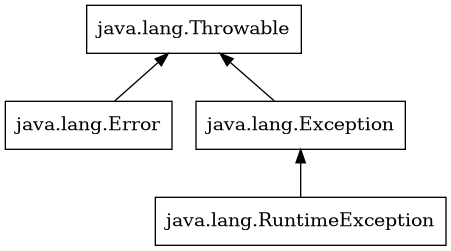
\includegraphics[scale=0.8]{coding/errorHandling/exception}
\end{center}

The different kinds of exceptions are discussed in \autocite{ORACLE_DOC_LANGUAGE_SPECIFICATION:KindsOfExceptions}.

Exception classes that extend \lstinline|java.lang.Exception|\index{java.lang!Exception} are so-called \textit{checked} exceptions\index{exception!checked exception}\index{checked exception|see{exception}}; a method\index{method} that may throw one of these must declare them with the \lstinline|throws| clause. The class \lstinline|java.lang.RuntimeException|\index{java.lang!RuntimeException} is a direct subclass of \lstinline|java.lang.Exception|\index{java.lang!Exception} and the superclass of all \textit{runtime}\index{runtime exception|see{exception}} or \textit{unchecked}\index{exception!unchecked exception}\index{unchecked exception|see{exception}} exceptions. It is not mandatory for a method\index{method} to declare them, but recommended.

While an ordinary program can \textit{potentially} recover from an error condition signalled by an \lstinline|Exception|\index{java.lang!Exception}\index{exception} instance, it is assumed that instances of the class \lstinline|java.lang.Error|\index{java.lang!Error}\index{exception!error} and its subclasses will indicate unrecoverable error conditions, causing the whole program or application to abort, not only the current operation.

This topic has various dimensions:
\begin{itemize}
	\item{The selection of the exception\index{exception} type to throw to report an error condition}
	\item{Catching exceptions\index{exception} and handling them}
	\item{Generating and throwing exceptions\index{exception}}
\end{itemize}


%------------------------------------------------------------------------------

\subsection{Which Exception to throw?}
When your code needs to issue an exception\index{exception} to signal an Error or a Failure, you must choose the respective exception\index{exception} class\index{class!exception class}. That selection gives already some basic information about the kind and origin of the problem, through the name of the exception\index{exception} class\index{class!exception class}, but also through the package that class belongs to. This means that the classes

\begin{itemize}[nosep]
	\item{\lstinline|java.lang.Throwable|\index{java.lang!Throwable} \autocite{ORACLE_DOC_THROWABLE_CLASS}}
	\item{\lstinline|java.lang.Exception|\index{java.lang!Exception} \autocite{ORACLE_DOC_EXCEPTION_CLASS}}
	\item{\lstinline|java.lang.RuntimeException|\index{java.lang!RuntimeException} \autocite{ORACLE_DOC_RUNTIMEEXCEPTION_CLASS}}
	\item{\lstinline|java.lang.Error|\index{java.lang!Error} \autocite{ORACLE_DOC_ERROR_CLASS}}
\end{itemize}

are forbidden, because they are too generic (and they are causing issues when catching\index{try!catch} exceptions\index{exception} what we will discuss later).

The class of the thrown exception should be chosen appropriate to the error condition it indicates. When scanning the Javadoc for the \Java Runtime Library \autocite{ORACLE_DOC_OVERVIEW}, you may find several exceptions\index{exception} with names that may fit for your purpose, but when you look after their package, they belong to an area that is by no means related to your method\index{method}.

Currently, our \lstinline|textToNumber()| method\index{method} from above throws the forbidden exception\index{exception} \lstinline|java.lang.RuntimeException|\index{java.lang!RuntimeException}. We want to fix that and we search the documentation for already existing exceptions\index{exception} that fits. Among others, we find the class \lstinline|javax.xml.crypto.dsig.TransformException|\index{javax.xml.crypto.dsig!TransformException} \autocite{ORACLE_DOC_TRANSFORMEXCEPTION_CLASS}; while the name \bdq{\texttt{TransformException}} sounds good, but our code is in no way related to XML processing or even some cryptology stuff so we should not use that exception to signal the failure of our \lstinline|textToNumber()| method. The exception of choice would be \lstinline|java.lang.NumberFormatException|\index{java.lang!NumberFormatException} \autocite{ORACLE_DOC_NUMBERFORMATEXCEPTION_CLASS} that is also thrown by the \lstinline|Integer::parseInt| method.

In reality, however, it only makes sense in rare cases to reuse an exception\index{exception} declared by another library, including most exceptions from the \Java Runtime Library.

The few exceptions to this are:
\begin{itemize}
	\item{\lstinline|java.lang.IllegalArgumentException|\index{java.lang!IllegalArgumentException} \autocite{ORACLE_DOC_ILLEGALARGUMENTEXCEPTION_CLASS} – The base class of the so-called \bdq{Validation Exceptions}\index{validation exception}\index{exception}; we discusse this in more detail in chapter \tqfullvref{sec:ValidationExceptions}.}
	
	\item{\lstinline|java.lang.IllegalStateException|\index{java.lang!IllegalStateException}  – From the documentation \autocite{ORACLE_DOC_ILLEGALSTATEEXCEPTION_CLASS}: \bdq{\textit{Signals that a method has been invoked at an illegal or inappropriate time. In other words, the Java environment or Java application is not in an appropriate state for the requested operation.}}}

	\item{\lstinline|java.lang.UnsupportedOperationException|\index{java.lang!UnsupportedOperationException} \autocite{ORACLE_DOC_UNSUPPORTEDOPERATIONEXCEPTION_CLASS} – It should be thrown in cases the requested operation is not supported. It is also used when a method from an interface\index{interface} is not (yet) implemented.}
\end{itemize}

As a rule of thumb, a failed check of a method's argument should throw a validation exception\index{validation exception}, as described on page \pageref{sec:ValidationExceptions}\footnote{\lstinline|java.lang.NumberFormatException|\index{java.lang!NumberFormatException} is extending \lstinline|java.lang.IllegalArgumentException|\index{java.lang!IllegalArgumentException}; that makes it a \bdq{validation exception}\index{validation exception}, and therefore we may use it for our \lstinline|textToNumber()| implementation.}.

For all other error conditions, it is recommended to create your own, domain-specific exceptions\index{exception} instead of re-using already existing exception classes\index{class!exception class}, as described in chapter \tqfullvref{sec:DomainSpecificExceptions}.

Obviously the name of the thrown exception\index{exception} should somehow correlate with the error condition it reports.

%------------------------------------------------------------------------------

\subsection{Catching Exceptions}
First, your production code may never contain a \lstinline|catch| clause\index{try!catch} for 
\begin{itemize}[nosep]
	\item{\lstinline|java.lang.Throwable|\index{java.lang!Throwable} \autocite{ORACLE_DOC_THROWABLE_CLASS}}
	\item{\lstinline|java.lang.Exception|\index{java.lang!Exception} \autocite{ORACLE_DOC_EXCEPTION_CLASS}}
	\item{\lstinline|java.lang.RuntimeException|\index{java.lang!RuntimeException} \autocite{ORACLE_DOC_RUNTIMEEXCEPTION_CLASS}}
	\item{\lstinline|java.lang.Error|\index{java.lang!Error} \autocite{ORACLE_DOC_ERROR_CLASS} and any of its subclasses}
	\item{\lstinline|java.lang.NullPointerException|\index{java.lang!NullPointerException} \autocite{ORACLE_DOC_NULLPOINTEREXCEPTION_CLASS}}
\end{itemize}

In this context, you should refer to the chapter \tqfullvref{sec:ExceptionHandlingInThreads} that explains why do you never need \lstinline|catch| clauses\index{try!catch} for \lstinline|Throwable|\index{java.lang!Throwable}, \lstinline|RuntimeException|\index{java.lang!RuntimeException} or \lstinline|Error|\index{java.lang!Error}.

There must be a dedicated \lstinline|catch|\index{try!catch} block for each exception\index{exception} that you want to handle; if code int the \lstinline|catch|\index{try!catch} block is the same for multiple exceptions, you list the exceptions\index{exception} in the \lstinline|catch|\index{try!catch} clause:
\keeplisting{3}
\begin{lstlisting}
try
{
    …
}
catch( final ABCException | DEFException | XYZException e ) { … }
\end{lstlisting}

There are only four reasons why your code contains a \lstinline|catch|\index{try!catch} block for a particular exception\index{exception}:
\begin{enumerate}
	\item{The \lstinline|catch|\index{try!catch} block can \bsq{heal} the error condition somehow. This can be done by using a default value instead of the result of the failed operation, or by retrying the operation. See chapter \tqfullvref{sec:GeneralExceptionHandling} for more details.}
	
	\item{The \lstinline|catch|\index{try!catch} block will externalise the error condition indicated by the caught exception\index{exception}; chapter \tqfullvref{sec:ReportFailure} will provide the details. Usually the current operation must be aborted afterwards.}
	
	\item{The caught exception\index{exception} must be enhanced and/or wrapped; this will discussed in more detail in chapter \tqfullref{sec:ThrowingExceptions}, \hyperref[sec:ThrowingExceptions]{below}. As a rule of thumb, each method that has parameters should catch all exceptions and enhance them with the arguments it was called with.}
	
	\item{The Java syntax rules require a \lstinline|catch|\index{try!catch} block (or a \lstinline|throws| declaration) despite it is impossible that the respective exception\index{exception} is ever thrown. Chapter \tqfullvref{sec:ImpossibleExceptions} will cover this topic.}
\end{enumerate}

In any other case, you let an exception\index{exception} \bsq{\textit{bubble up}} – meaning your code does not have a \lstinline|catch|\index{try!catch} clause at all and delegates the handling of the exception\index{exception} to the caller. In case of checked exceptions\index{exception!checked exception}, your method must declare each exception\index{exception} in a \lstinline|throws| clause. 
 
%------------------------------------------------------------------------------

\subsection{General Exception Handling}\label{sec:GeneralExceptionHandling}

\bdq{To handle an exception\index{exception}} means to restore the program state to normal. If a method\index{method} is unable to recover from an error condition indicated by an exception\index{exception}, it must delegate it to its caller.

Delegation can be done either by ignoring the exception – in this case it will be propagated to the caller automatically (it \bdq{\textit{bubbles up}}) – or by catching and wrapping it, as described in chapter \tqfullref{sec:ThrowingExceptions}.

\bdq{Restoring the program state to normal} or \bdq{healing the error condition} can be achieved in various ways, also depending on the context. For the examples below it would be often possible to avoid the exception\index{exception} completely by coding it differrently (e.g. by checking the conditions upfront, as shown on page \pageref{lbl:ValidateInput}). I used exceptions\index{exception} to illustrate the topic.

\paragraph{Example~1} The method below should create an instance of \lstinline|java.io.Writer|\index{java.io!Writer} for an already existing file; we assume that the argument was checked to be not \lstinline|null| before the call to \lstinline|openOutputFile|.

A \lstinline|FileNotFoundException|\index{java.io!FileNotFoundException} is thrown in line~7 when the specified file or the path for that file does not exist, but instead of delegating that back to the caller, we catch that exception\index{exception} in line~9, create the directory for the file and the file itself, before we initialise it by writing the file header to the \lstinline|Writer|\index{java.io!Writer} instance. 

Other variants of \lstinline|java.io.IOException|\index{java.io!IOException} are still delegated to the caller; they could be thrown in lines~7, 11, 12 and 13.

\keeplisting{15}
\index{java.io!Writer}\index{java.nio.file.Path}\index{java.io!IOException}\index{java.nio.file!Files}\index{java.nio.file!Files!newBufferedWriter()}\index{java.io!FileNotFoundException}\index{java.nio.file!Files!createDirectories()}\index{java.nio.charset!StandardCharsets!UTF\_8}\index{java.nio.file!StandardOpenOption!APPEND}\index{java.nio.file!StandardOpenOption!CREATE\_NEW}\index{java.nio.file!StandardOpenOption!WRITE}
\begin{lstlisting}
private final Writer openOutputFile( final Path existingFile ) throws IOException
{
    Writer retValue;
    try
    {
        retValue = Files.newBufferedWriter( existingFile, UTF_8, WRITE, APPEND );
    }
    catch( final FileNotFoundException _ )
    {
        Files.createDirectories( existingFile.getParent() );
        retValue = Files.newBufferedWriter( existingFile, UTF_8, WRITE, CREATE_NEW );
        writeHeader( retValue );
    }

    //---* Done *----------------------------------------------------------
    return retValue;
}   //  openOutputFile()
\end{lstlisting}

\paragraph{Example 2} This method should establish a connection to an external system. After checking the arguments in lines~3 and 4, an attempt is made to instantiate a new \lstinline|Socket|\index{java.net!Socket} object in a loop. If that attempt is successful, the loop will be left (line~13), the \lstinline|Socket|\index{java.net!Socket} instance is wrapped in an instance of \lstinline|Optional|\index{java.util!Optional} (line~23) that is returned afterwards.

If the instantiation of the new \lstinline|Socket|\index{java.net!Socket} fails with an \lstinline|UnknownHostException|\index{java.net!UnknownHostException} or a \lstinline|ConnectException|\index{java.net!ConnectException}, the method waits for 30~seconds (line~17), increments the \lstinline|retryCounter| and continues the loop until the \lstinline|retryCounter| is greater than \lstinline|maxRetries|, another exception than \lstinline|UnknownHostException|\index{java.net!UnknownHostException} or \lstinline|ConnectException|\index{java.net!ConnectException} is thrown, or an attempt to instantiate the socket instance was successful.

\lstinline|Thread::sleep| may throw an \lstinline|InterruptedException|\index{java.lang!InterruptedException} that will also abort the method.
 
\keeplisting{25}
\begin{lstlisting}
public final Optional<Socket> connect( final InetAddress address, final int port, final int maxRetries ) throws InterruptedException, IOException
{
    if( isNull( address ) ) throw new IllegalArgumentException( "address is null" );
    if( (port < 0) || (port > 0xFFFF) ) throw new IllegalArgumentException( "port is invalid: %d".formatted( port ) ); 
    
    Socket socket = null;
    var retryCounter = 0;
    ConnectLoop: while( retryCounter < max( 1, maxRetries ) )
    {
        try
        {
            socket = new Socket( address, port );
            break ConnectLoop;
        }
        catch( final UnknownHostException | ConnectException _ )
        {
            sleep( ofSeconds( 30 ) );
            socket = null;
            ++retryCounter;
        }
    }   //  ConnectLoop:

    final Optional<Socket> retValue = Optional.ofNullable( socket );

    //---* Done *----------------------------------------------------------
    return retValue;
}   //  connect()
\end{lstlisting}

This method is clearly using the exceptions\index{exception} to control the execution flow – something that usually should be avoided. Unfortunately, the \Java Runtime Library does not provide an API to check the availability of an external system that does not rely on exceptions\index{exception}.

\paragraph{Example 3}
















%------------------------------------------------------------------------------

\subsection{Throwing Exceptions}\label{sec:ThrowingExceptions}
We discussed already \hyperref[sec:ExceptionCosts]{above} that throwing an exception\index{exception} should be done with some care, because it will have its price.

Invalid arguments for a method\index{method} must be signalled by throwing a validation exception\index{validation exception} as described in chapter \tqfullvref{sec:ValidationExceptions}. The message for these exceptions contains the name of the parameter, the invalid argument, and the reason why that is invalid. The latter is often already indicated by the type of the thrown exception: when \lstinline|Integer::parseInt|\index{java.lang!Integer!parseInt()} throws a \lstinline|NumberFormatException|\index{java.lang!NumberFormatException}, it is obvious that the given argument cannot be parsed to a number because it contains invalid characters.

When execution failures should be reported through an exception\index{exception}, this exception\index{exception} is not necessarily thrown explicitly by the current code – it could be be easily originate from a method\index{method} that was called by the current method and is just delegated. Whether this is sufficient depends from the context and the type of product you work on.

But for \hyperref[sec:FeatureLibrary]{feature libraries}\index{product type!feature library} as well as for \hyperref[sec:StandaloneApplication]{standalone applications}\index{product type!standalone application} and \hyperref[sec:ServerbasedApplication]{server-based applications}\index{product type!server-based application} with multiple modules, you must ensure that a method\index{method} at the domain (or module) boundaries will emit only domain-specific exceptions\index{domain-specific exception} for execution failures; it is not mandatory that validation exceptions\index{validation exception} are domain-specific.

That means that a method that is part of the public API of a module must catch all exceptions and wrap them into a domain-specific exception\index{domain-specific exception}, enhanced by a proper exception message that provides the  context for the error condition. This consists of a short description of what was attempted with the failed operation, together with the relevant arguments of the current method. If the failed operation itself signalled the error condition through an exception\index{exception}, this exception must be part of the wrapper exception, too, as the \bdq{cause}. Otherwise, the arguments of the failed call should be part of the exception message, too. Same if the caught exception does not contain these arguments.

But also within a module it could be necessary to catch an exception\index{exception} and to wrap it, in order to keep the context of the call. As a rule of thumb, each method\index{method} that has parameters should catch all exceptions\index{exception} and enhance them with the arguments it was called with.

\keeplisting{10}
For a method with the signature \bdq{\lstinline|aMethod( final String recipientId, final String dataSource )|} wrapping looks like this:
\begin{lstlisting}
try
{
    …
}
catch( final AnException e ) 
{
    throw new DomainException( """
```````Printing Operation failed
```````Recipient Id: %s
```````Origin: %s
```````""".formatted( recipientID, dataSource ), e;
}
\end{lstlisting}

The name of the method (here \lstinline|aMethod|) must not be part of the exception\index{exception} message as it is already provided through the stack trace stored with the exception\index{exception} object.

%------------------------------------------------------------------------------








When selecting the exception class, your first look should be to the already existing exception implementations if there is already one that fits your needs.\footnote{Although sometimes the name of an exception looks good, you should also consider which package it lives in; throwing an exception from a JNDI related package like \lstinline|javax.naming.OperationNotSupportedException|\index{javax.naming!OperationNotSupportedException} in a code segment that does nothing with the \bdq{Java Naming and Directory Interface} at all will cause more confusion than it helps. Not to mention that it may require an additional module.} If none of the existing ones fit, implement your one exception class by extending one of \lstinline|Exception|\index{java.lang!Exception}, \lstinline|RuntimeException|\index{java.lang!RuntimeException}, or \lstinline|Error|\index{java.lang!Error}, depending on your needs\footnote{You can create your own exception class that extends \lstinline|Throwable|\index{java.lang!Throwable} directly, but so far I have not found a use case for that.}. This is always useful in the case of a feature library to simplify its API\footnote{All methods will only throw one exception especially created for that library, or exceptions derived from that. Samples for this pattern are the Servlet API (throwing only instances of \lstinline|IOException|\index{java.io!IOException} and \lstinline|ServletException|\index{javax.servlet!ServletException}) or JDBC (throwing only \lstinline|SQLException|\index{java.sql!SQLException} instances).}, and it can be also helpful for an application.

When implementing an extension or a server-based application (or when using a particular framework), you have to implement quite often methods that declare only one, sometimes two exceptions. Nevertheless, it may happen that a method call in your code throws an exception that cannot be handled by the current code, but it cannot be delegated also, because the interface for the method does not declare that particular exception. In such a case, you have to catch the exception and to wrap it into an instance of the declared exception that will be thrown afterwards. For a servlet implementation\autocite{JAKARTA_EE_HTTPSERVLET_CLASS}, this may look like this:
\begin{lstlisting}
protected final void doGet( HttpServletRequest request, HttpServletResponse response )
    throws ServletException, IOException
{
    …
    try
    {
        …
    }
    catch( final TimeOutException e )
    {
        throw new ServletException( e );
    }

    …
}  //  doGet()
\end{lstlisting}

When instantiating an exception instance, you should always provide a textual message that describes the error condition and/or provides additional information, like the name of the file that cannot be found, or the SQL statement with the invalid syntax.\footnote{In this regard, the sample above is bad, because it does not provide such an explanation.} These text have to be in English language, for the same reason why the names and the comments are in English.

Of course, messages that will be presented to the end user in a UI have to be localised, but the UI should not display the raw exception message anyway at all.

Some exception classes do not have a constructor that allows to provide a cause, or they have constructors that allow either a message or a cause, but not both. A sample for that is \lstinline|java.lang.ExceptionInInitializerError|\autocite{ORACLE_DOC_EXCEPTIONININITIALIZERERROR_CLASS}.

Some of these exception classes will allow a workaround that allows you to still provide both, cause and message, with them, like below:\footnote{Unfortunately, \lstinline|ExceptionInInitializerError| does not belong to this group of exception classes.}: 
\begin{lstlisting}
static
{
    try
    {
        …    
    }
    catch( final Exception e )
    {
        throw new DumpException( "Message" )
            .initCause( e );    
    }
}
\end{lstlisting}

For the method \lstinline|initCause()| refer to \autocite{ORACLE_DOC_THROWABLE:initCause}.

Unfortunately, you have to test whether the exception that you have to deal with allows this workaround. And you should add this test to the unit tests\index{unit test} for your code, to protect you from changes coming with new versions.













































Each exception that is thrown by 

Basically, a method\
A method\index{method} signals an error by emitting an exception, but 

 
Exceptions\index{exception} are thrown 

Although not explicitly said in the chapter above, it should be obvious that the















If the domain specific exception would allow to add information to it, that could look like this:
try
{
    …
}
catch( final DomainException e ) 
{
    e.addInfo( "Message", "Printing Operation failed" );
    e.addInfo( "Recipient Id", recipientID );
    e.addInfo( "Origin", dataSource ); 
    throw e;
}
“Handling an Exception” usually means that the error condition that caused the exception is removed or healed. Whether or not the exception is logged depends on the circumstances, but it must be obvious that it will never be logged with ERROR or FATAL when the error condition has gone!
Exceptions may never be swallowed. This means that code like this is inherently wrong or illegal:
\begin{lstlisting}
try
{
    …
}
catch( final AnException _ ) {}
\end{lstlisting}
Nonetheless, it is possible that you do not need to handle a caught exception, either because the system is not in an error state despite the exception (perhaps because you already provided a default value that is used in case the retrieval of a config value fails), or the exception is declared for a method called from the try block, but cannot be thrown by that method. You must provide at least a comment in the otherwise empty block:
\begin{lstlisting}
catch( final AnException _ ) { /* Deliberately ignored */ }
\end{lstlisting}
Or, better, with an explanation: 
\begin{lstlisting}
catch( final AnException _ ) { /* Default value is used in case of failure */ }
\end{lstlisting}
In the second case, you should consider throwing a dedicated exception:
catch( final AnException e ) { throw new ImpossibleExceptionError( e ); }
This protects the code a little bit from changes to the implementation of the method that previously could not throw the exception. At least the Exception will not go unnoticed when thrown.
Another recommendation regarding Error handling is that it must not obscure the essentials. When you write the code that checks for an error condition or handles an error condition, come to the point fast, otherwise the readability of the code suffers.
The finally Block
The complete syntax for the exception handling is try-catch-finally:
\begin{lstlisting}
try
{
    …
}
catch( final AnException e ) { … }
finally
{
    // Some code
    …
}
\end{lstlisting}
The JVM guarantees that the code in the finally block will be executed under all circumstances, no matter how the try block is left.3
This is used for code like this:
theLock.lock(); // Retrieve the lock
try
{
    // Do something that needs synchronisation
    …
}
catch( final AnException e ) { … }
finally
{
    theLock.unlock(); // Release the lock
}
Unfortunately, we had INCs regarding locks that were held by already terminated threads. The interpretation was that there must be a bug in the JVM that, under some circumstances, allows a thread to terminate without executing a finally block.
But the solution was much more profane: there was code before the call to Lock::unlock that threw an exception so that the finally block was left before unlock() was called at all. 
The specification says that the code in the finally block is always executed, but it does not state that the code block is always left on its end or that the code is executed completely.
Consequently, all the housekeeping chores should be done at the very beginning of the finally block, with those calls first that cannot fail with an exception.






















Only the method’s name is not needed as this is part of the stack trace stored with the exception itself.
Not all exceptions that are emitted by a method are explicitly thrown by it! A RuntimeException (an unchecked exception) thrown by a method called by the current method may bubble up to the caller if that current method, same as a checked exception that is declared to be thrown by the current method.
To allow a specific handling of the emitted exceptions, each method must declare all of them (including the unchecked ones!), in a detailed list; a mere “throws Exception” is wrong!
Your method should fail fast, if at all. This means that all checks should be placed to the beginning of a method, and that an operation is aborted immediately after an unrecoverable error condition is identified.
This also means that each method (in Pega, this includes the Rules) must check immediately its arguments whether they are valid, and that it must throw a “validation exception” (an exception that is derived from IllegalArgumentException) in case that check fails.

\subsection{Exception Handling in Threads}
The most often heard excuse for a catch phrase for java.lang.RuntimeException, java.lang.Exception or even java.lang.Throwable is that exceptions thrown while executing a thread that is not the main thread may not go unnoticed. So you see code like this:
public final void run()
{
    try
    {
        // Do whatever this thread must do …
    }
    catch( final Exception e )
    {
        oLog.error( "No matter what went wrong, but I will log the exception", e );
    }
} 
Unfortunately, this absolves the programmer of the duty to properly handle any exceptions thrown within the try block; the catch block at the end will take care of it.
The best practice is to set the UncaughtExceptionHandler for the thread, either through the ThreadFactory, through the ThreadGroup or individually. If your thread requires a special handling for an uncaught exception, this looks like below; the sample assumes that the thread comes from a pool and is reused:
public final void run()
{
    final var currentThread = Thread.currentThread();
    final var uncaughtExceptionHandler = currentThread.getUncaughtExceptionHandler();
    currentThread.setUncaughtExceptionHandler( (t,e) ->
    {
        /*
         * The special exception treatment goes here …
         *

        // Finally log the exception
        oLog.fatal( """
            Thread "%s" was aborted with an exception!\
            """.formatted( t.getName() ), e );
    } );
 
    try
    {
        // Do whatever this thread must do …
    }
    finally
    {
        currentThread.setUncaughtExceptionHandler( uncaughtExceptionHandler );
    }
}
But usually a thread should use the UncaughtExceptionHandler that is assigned through the factory or group, as already said, or you even define a default handler. All this needs to be regulated by a proper guide to exception Handling that needs to be defined.
























To handle an exception you first have to catch it.

Catching \lstinline|java.lang.Exception| is discouraged in most cases; it \textit{can} be acceptable when you need to wrap all checked exceptions into a runtime exception or into an error:
\begin{lstlisting}
public final void run()
{
    try
    {
        …
    }
    catch( final Exception e )
    {
        throw new WrapperException( e );
    }
}   // run()
\end{lstlisting}

You should absolutely avoid to catch \lstinline|java.lang.Error| and all of its subclasses, \lstinline|java.lang.RuntimeException|, and of course, you should not never ever catch \lstinline|java.lang.Throwable|\index{java.lang!Throwable}!\footnote{But no rule without an exception: refer to chapter \tqvref{sec:ExceptionHandlingInThreads}.}

Provide a \lstinline|catch| block for each and every exception that you want to handle:
\begin{lstlisting}
public final void run()
{
    try
    {
        …
    }
    catch( final FileNotFoundException e )
    {
        throw new ApplicationError( "Cannot find file", e );
    }
    catch( final IOException e )
    {
        throw new ApplicationError( "An error occurred on processing the input file", e );
    }
    catch( final NumberFormatException e )
    {
        throw new ApplicationError( "Input Data is corrupted", e );
    }
    catch( final PatternSyntaxException e )
    {
        throw new ApplicationError( "Pattern invalid", e );
    }
}   // run()
\end{lstlisting}

Sometimes when a large number of exceptions has to be handled with all the same code, you may be tempted to just catch \lstinline|java.lang.Exception|. As already said: don't do it! This approach will definitely cause problems as it may handle runtime exceptions in the same \lstinline|catch|-block as the checked exceptions, and usually this is not intended.

A simplificatin for the sample above could look like this:
\begin{lstlisting}
public final void run()
{
    try
    {
        …
    }
    catch( final IOException | NumberFormatException | PatternSyntaxException e )
    {
        throw new ApplicationError( "Processing failed", e );
    }
}   // run()
\end{lstlisting}
Still only the declared exceptions will be handled in the \lstinline|catch|-block, but unexpected exceptions will now bubble up\footnote{The exception class \lstinline|java.io.FileNotFoundException| is not listed because its superclass \lstinline|java.io.IOException| is already on the list.}.

Sometimes an exception indicates a regular program state (although this would indicate poor design in most cases)\footnote{Nevertheless, you can find this even in the Java Runtime Library~… but no one has ever said that the authors of the JDK had never made doubtful decisions.}. Usually you will avoid this situation by e.g. checking the operands before an operation, but a very popular example where this is not practicable is the conversion of a string into a numerical value:
\begin{lstlisting}
…
var amount = 0.0;
final var requestParam = request.getParameter( "amount" );
try
{
    if( nonNull( requestParam ) )
    {
        amount = Double.parseDouble( requestParam );
    }
}
catch( final NumberFormatException ignored )
{
    //---* If amount in request is not numeric, set it to 0.0 *------
    amount = 0.0;
}
…
\end{lstlisting}

As shown in the example, a comment is required in the catch clause, because you do not further propagate the exception neither do you log it.

It is also possible that you checked the preconditions, but you still have to deal with some checked exceptions:
\begin{lstlisting}
…
final var file = new File( … );
if( file.exists() )
{
    try( final var input = new FileInputStream( file ) )
    {
        …
    }
    catch( final FileNotFoundException e )
    {
        throw new UnexpectedExceptionError( "File was there when checked!", e );
    }
}
…
\end{lstlisting}

A sample for the class \lstinline|UnexpectedExceptionError| can be found in \autocite{TQUADRAT_ORG_FOUNDATION_UNEXPECTEDEXCEPTIONERROR}.

Some APIs in the JDK declares a checked exception, but that will never be thrown for the given arguments by any means. Most famous for this are the conversions from byte arrays to Strings and back:
\begin{lstlisting}
…
final String s;
try
{
    s = new String( byteArray, "UTF-8" );
}
catch( final UnsupportedEncodingException e )
{
    throw new ImpossibleExceptionError( "UTF-8 must exist!", e );
}
…
\end{lstlisting}

According to \autocite{ORACLE_DOC_CHARSET:StandardCharsets}, the UTF-8 encoding is mandatory for each JDK/JVM implementation, therefore the code sequence above will \textit{never} throw an \lstinline|UnsupportedEncodingException|. Nevertheless, it is not allowed to swallow the exception; instead an error should be thrown in the \lstinline|catch| clause, indicating the error condition. In the improbable case UTF-8 is not supported by the current Java runtime environment, the problem will surface, and the program will not die silently without any hint about the reason.\footnote{If, of course, there is no catch for \lstinline|Throwable| somewhere on the path.} It also protects you from malicious changes to the name of the character encoding: a none existing \lstinline|Charset| will cause noise.

Of course, the problem could be solved differently, by using an instance of \lstinline|java.nio.charset.Charset|\autocite{ORACLE_DOC_CHARSET_CLASS} as the argument to the \lstinline|String| constructor, instead of the name of the character encoding. For this case, the constructor does not declare an \lstinline|UnsupportedEncodingException|. 

Another example is the interface \lstinline|java.lang.Appendable|\autocite{ORACLE_DOC_APPENDABLE_INTERFACE}: it is implemented by \lstinline|java.io.Writer| and \lstinline|java.io.PrintStream|, but also by \lstinline|java.lang.StringBuilder| (and a few more). The method \lstinline|java.lang.Appendable::append| declares to throw an \lstinline|IOException|, but the implementation of that method for \lstinline|StringBuilder| will never throw it and does not even declare it.
\begin{lstlisting}
…
final Appendable appendable = new StringBuilder();
try
{
    appendable.append( "Some Text" );
}
catch( final IOException e )
{
    throw new ImpossibleExceptionError( "Append to StringBuilder", e );
}
…
\end{lstlisting}

Again, a sample for \lstinline|ImpossibleExceptionError| can be found in \autocite{TQUADRAT_ORG_FOUNDATION_IMPOSSIBLEEXCEPTIONERROR}.

Sometimes a method wants to act upon an error condition without handling the exception. In this case, it may catch the exception, does whatever necessary, then throw it again. An example:
\begin{lstlisting}
public final void myMethod() throw IOException
{
    final Predicate<String> isNetworkError = m_NetworkErrorPattern.asMatchPredicate();
    …
    try
    {
        …
    }
    catch( final IOException e )
    {
        final var message = e.getMessage();
        if( nonNull( message ) && isNetworkError.test( message ) ) ++networkErrors;
        throw e;
    }
    …
}   // myMethod()
\end{lstlisting}

It is usually not a good idea to log an exception and to rethrow or to wrap it afterwards, because this might cause the exception to be logged twice (or even more often). More details about logging can be found in chapter \tqvref{sec:Logging}.

Finally, you handle the exception somehow, by assigning a default value\footnote{see the sample about the conversion from string to number, above.}, or by performing an alternative action. In any case, you need to provide a comment in the \lstinline|catch| why you do not further delegate the handling of the exception.

If an exception was not caught in your code, it ”bubbles up” until it reaches the main method for the current thread (that is \lstinline|main()| for the main or program thread, and \lstinline|run()|\autocite{ORACLE_DOC_RUNNABLE:run} for any other thread). If this method will not handle the exception, the thread will be aborted. If this thread is the last non-deamon thread, the JVM will be terminated, too.

%==============================================================================
% End of file!!
%==============================================================================


\section{Exception Handling in Threads}\label{sec:ExceptionHandlingInThreads}
When we execute the Java program below, the \lstinline|Error|\index{java.lang!Error} is printed to the console:
\lstinputlisting{coding/errorHandling/TestAbortMain.java}

%\begin{verbatim}
%$ java TestAbortMain.java
%Exception in thread "main" java.lang.Error: Aborted
%	at TestAbortMain.main(TestAbortMain.java:5)
%$ 
%\end{verbatim}

\begin{center}
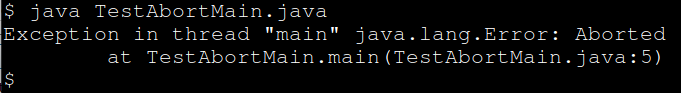
\includegraphics[scale=0.6]{coding/errorHandling/TestAbortMain}
\end{center}

In the sample below, we abort a secondary thread:
\lstinputlisting{coding/errorHandling/TestAbortThread.java}

When executed with contemporary versions of Java, the output will look like the screenshot below; for older versions of Java (before Java~5), there wouldn't be shown any output from the thread at all:






\chapter*{Road Work ahead!}








%\begin{verbatim}
%$ java TestAbortRun.java
%Exception in thread "Thread-0" java.lang.Error: run() aborted!
%	at TestAbortRun.run(TestAbortRun.java:5)
%	at java.base/java.lang.Thread.run(Thread.java:1474)
%Exception in thread "main" java.lang.Error: main() aborted!
%	at TestAbortRun.main(TestAbortRun.java:20)
%$ 
%\end{verbatim}

\begin{center}
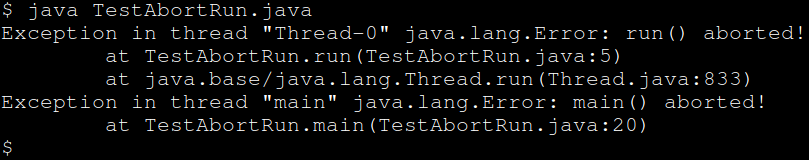
\includegraphics[scale=0.5]{coding/errorHandling/TestAbortRun}
\end{center}

\chapter*{Road Work done!}


This behaviour can be sufficient for a tool\index{product type!tool} (see chapter \tqref{sec:Tool} on page \pageref{sec:Tool}) or a script (chapter \tqref{sec:ScriptInJava} on page \pageref{sec:ScriptInJava}), but it is not feasible for a standalone application\index{product type!standalone application} (chapter \tqref{sec:StandaloneApplication} on page \pageref{sec:StandaloneApplication}) and not for a feature library\index{product type!feature library} (chapter \tqref{sec:FeatureLibrary} on page \pageref{sec:FeatureLibrary}).

A function library\index{product type!function library} (chapter \tqref{sec:FunctionLibrary} on page \pageref{sec:FunctionLibrary}) usually relies for the reporting of error conditions on the caller of a method\index{method}, while server-based applications\index{product type!server-based application} (chapter \tqref{sec:ServerbasedApplication} on page \pageref{sec:ServerbasedApplication}) and extensions\index{product type!extension} (chapter \tqref{sec:Extension} page \pageref{sec:Extension}) use the facilities provided by the host applications for this purpose.

For both a standalone application\index{product type!standalone application} and for a feature library\index{product type!feature library}, you want that error conditions will be tracked somehow\footnote{usually this means logging - see chapter \tqfullvref{sec:Logging}}, under all circumstances, and from all threads – because no error may go unnoticed, as required in the \ngref, bullet point~\ref{lst:ZoP:ErrorsMayNeverBeSwallowed}.

The payload of a thread\index{thread} is an implementation of the method \lstinline|run()|\index{java.lang!Runnable!run()} \autocite{ORACLE_DOC_RUNNABLE:run} from the interface \lstinline|java.lang.Runnable|\index{java.lang!Runnable} \autocite{ORACLE_DOC_RUNNABLE_INTERFACE}. 

You find quite often code in such implementations that follows the pattern shown below. Sometimes a \lstinline|catch|\index{try!catch} clauses for \lstinline|java.lang.RuntimeException|\index{java.lang!RuntimeException}, or even \lstinline|java.lang.Throwable|\index{java.lang!Throwable} are used, instead of one for \lstinline|java.lang.Exception|\index{java.lang!Exception}.

\keeplisting{7}
\index{java.lang!Exception}
\begin{lstlisting}
// DISCOURAGED!!
public final void run()
{
    try
    {
        // Do whatever this thread must do …
    }
    catch( final Exception e ) // DON'T CATCH EXCEPTION!!!
    {
        m_Logger.error( "No matter what went wrong, but I will log the exception", e );
    }
} 
\end{lstlisting}

This is a very bad excuse for a \lstinline|catch|\index{try!catch} clause for \lstinline|Exception|\index{java.lang!Exception}, \lstinline|RuntimeException|\index{java.lang!RuntimeException} or \lstinline|Throwable|\index{java.lang!Throwable}!

This is so bad because this code pattern absolves the programmer of the duty to properly handle any exceptions\index{exception} thrown within the \lstinline|try|\index{try} block individually – with a \lstinline|catch|\index{try!catch} clause for \lstinline|java.lang.Exception|\index{java.lang!Exception} even including the checked\index{exception!checked exception} ones – because the \lstinline|catch|\index{try!catch} block at the end will take care of all exceptions.

The best practice here is to set the \bdq{Uncaught Exception Handler}\index{java.lang!Thread.UncaughtExceptionHandler} \autocite{ORACLE_DOC_UNCAUGHTEXCEPTIONHANDLER_INTERFACE} for the thread\index{thread}, either through the \lstinline|ThreadFactory|\index{java.util.concurrent!ThreadFactory} \autocite{ORACLE_DOC_THREADFACTORY_INTERFACE}, through the \lstinline|ThreadGroup|\index{java.lang!ThreadGroup} \autocite{ORACLE_DOC_THREADGROUP_CLASS} or individually. 

\keeplisting{1}
\lstinline|java.lang.Thread.UncaughtExceptionHandler|\index{java.lang!Thread.UncaughtExceptionHandler} is a functional interface\index{interface!functional interface} that can be easily implemented as a method\index{method} like this:
\begin{lstlisting}[caption=UncaughtExceptionHandler as Method]
private static final void uncaughtExceptionHandler( final Thread t, final Throwable e )
{
    final var throwableType = e instanceof Error ? "error" : "exception";
    final var message = """
````````Thread "%s" was aborted with an %s!\
````````""".formatted( t.getName(), throwableType ) 
    m_Logger.atFatal()
        .withThrowable( e )
        .log( message );    
}   //  uncaughtExceptionHandler()
\end{lstlisting}
When you need to set the uncaught exception handler\index{java.lang!Thread.UncaughtExceptionHandler}, you refer to that method with a method reference: \lstinline|<Class>::uncaughtExceptionHandler|.

Of course it can be implemented as a class as well:
\begin{lstlisting}[caption=UncaughtExceptionHandler as Class]
/**
 *  <p>{@summary An implementation for
 *  {@link UncaughtExceptionHandler}.}</p>
 */
public final class UncaughtExceptionHandlerImpl implements UncaughtExceptionHandler
{
        /*------------------------*\
    ====** Static Initialisations **======================================
        \*------------------------*/
    /**
     *  <p>{@summary The instance of this class.}</p>
     */
    public static final UncaughtExceptionHandler INSTANCE = new UncaughtExceptionHandlerImpl();

    /**
     *  <p>{@summary The logger that is used to log the exceptions.}</p>
     */
    private static final Logger m_Logger = getLogger( UncaughtExceptionHandler.class.getName() );

        /*--------------*\
    ====** Constructors **================================================
        \*--------------*/
    /**
     *  <p>{@constructor}}</p>
     */
    public UncaughtExceptionHandlerImpl() { /* Just exists */ }

        /*---------*\
    ====** Methods **=====================================================
        \*---------*/
    /**
     *  {@inheritDoc}
     */
    @Override
    public final void uncaughtException( final Thread t, final Throwable e )
    {
        final var throwableType = e instanceof Error ? "error" : "exception";
        final var message = """
````````````Thread "%s" was aborted with an %s!\
````````````""".formatted( t.getName(), throwableType ); 
        m_Logger.atFatal()
            .withThrowable( e )
            .log( message );    
    }   //  uncaughtException()
}
//  class UncaughtExceptionHandlerImpl
\end{lstlisting}

\keeplisting{1}
Or as an anonymous class\index{class!anonymous class}
\begin{lstlisting}[caption=UncaughtExceptionHandler as Anonyomous Class]
private static final UncaughtExceptionHandler = m_UncaughtExceptionHandler = new Thread.UncaughtExceptionHandler()
{
    /**
     *  {@inheritDoc}
     */
    @Override
    public final void uncaughtException( final Thread t, final Throwable e )
    {
        final var throwableType = e instanceof Error ? "error" : "exception";
        final var message = """
````````````Thread "%s" was aborted with an %s!\
````````````""".formatted( t.getName(), throwableType ); 
        m_Logger.atFatal()
            .withThrowable( e )
            .log( message );    
    }   //  uncaughtException()
};
\end{lstlisting}

\keeplisting{3}
Setting the uncaught exception handler\index{java.lang!Thread.UncaughtExceptionHandler} for an individual thread\index{thread} looks like this:
\begin{lstlisting}
Thread.ofPlatform()
    .group( threadGroup )
    .uncaughtExceptionHandler( this::uncaughtExceptionHandler )
    .start( () -> {…} );
\end{lstlisting}
Here the method \lstinline|uncaughtExceptionHandler()|is not static; that can be usefull when the failure message should depend on the instance.

\keeplisting{3}
For a thread pool\index{thread pool}, the code would be similar to this:
\begin{lstlisting}
final var factory = Thread.ofPlatform()
    .group( threadGroup )
    .uncaughtExceptionHandler( this::uncaughtExceptionHandler )
    .factory();
final var threadPool = Executors.newCachedThreadPool( factory );
\end{lstlisting}

If the uncaught exception handler\index{java.lang!Thread.UncaughtExceptionHandler} is provided by the \lstinline|ThreadGroup|\index{java.lang!ThreadGroup} instance, the call to \lstinline|Builder::uncaughtExceptionHandler|\index{java.lang!Thread.Builder!uncaughtExceptionHandler()} should be omitted; otherwise it overwrites the setting from the group.

A thread group is supported only by platform threads\index{thread!platform thread}, not by virtual threads\index{thread!virtual thread}. Additionally, the \lstinline|ThreadGroup|\index{java.lang!ThreadGroup} implementation provided by the \Java Runtime Library does not allow to set a custom uncaught exception handler. In chapter \tqref{sec:ThreadGroup} on page \pageref{sec:ThreadGroup} I show an implementation of \lstinline|ThreadGroup|\index{java.lang!ThreadGroup} that got that feature added.

Through the static method \lstinline|Thread::setDefaultUncaughtExceptionHandler|\index{java.lang!Thread!setDefaultUncaughtExceptionHandler()} \autocite{ORACLE_DOC_THREAD:setDefaultUncaughtExceptionHandler} you can even define a default handler that is used by all threads that does not specify an individual one, as shown in chapter \tqfullvref{sec:MethodMain}.

Usually a thread should use the \lstinline|UncaughtExceptionHandler|\index{java.lang!Thread.UncaughtExceptionHandler} that is assigned to it on creation. But if your method\index{method} requires a special treatment for an uncaught exception when executed within a thread from a thread pool, the method\index{method} can set an individual uncaught exception handler\index{java.lang!Thread.UncaughtExceptionHandler} as shown in the code sample below.

\index{java.lang!Runnable!run()}\index{java.lang!Thread!currentThread()}\index{java.lang!Thread!getDefaultUncaughtExceptionHandler()}\index{java.lang!Thread!setDefaultUncaughtExceptionHandler()}\index{java.lang!Thread.UncaughtExceptionHandler}
\begin{lstlisting}
public final void run()
{
    final var currentThread = Thread.currentThread();
    final var uncaughtExceptionHandler = currentThread.getUncaughtExceptionHandler();
    currentThread.setUncaughtExceptionHandler( (t,e) ->
    {
        /*
         * The special exception treatment goes here …
         *

        //---* Finally log the exception *--------------------------------
        m_Logger.fatal( () -> """
````````````````Thread "%s" was aborted with an exception!\
````````````````""".formatted( t.getName() ), e );
    } );
 
    try
    {
        /*
         * Do whatever this thread must do …
         */
    }
    finally
    {
        //---* Reset the uncaught exception handler *---------------------
        currentThread.setUncaughtExceptionHandler( uncaughtExceptionHandler );
    }
}   //  run()
\end{lstlisting}

That \bdq{special treatment} could be an individual message, but also that you want to log the issue in a different manner or to another location.

If your code changes the uncaught exception handler\index{java.lang!Thread.UncaughtExceptionHandler} of the thread that executes that code, it must restore the handler before it terminates, because threads from a thread pool are reused with different payloads (during their lifetime, they execute the \lstinline|run()|\index{java.lang!Runnable!run()} method from different instances of \lstinline|Runnable|\index{java.lang!Runnable} implementations). Although virtual threads\index{thread!virtual thread} are not reused\footnote{At least not if you follow the recommendations given in JEP~444 \autocite{JEP444:Pooling}.}, you should restore the uncaught exception handler\index{java.lang!Thread.UncaughtExceptionHandler} even when \lstinline|Thread::isVirtual|\index{java.lang!Thread!isVirtual()} \autocite{ORACLE_DOC_THREAD:isVirtual} returns \lstinline|true| for the current thread\index{thread}.

%==============================================================================
% End of file!!
%==============================================================================

\section{Unexpected and Impossible Exceptions}\label{sec:ImpossibleExceptions}
The interface \lstinline|java.lang.Appendable|\index{java.lang!Appendable} \autocite{ORACLE_DOC_APPENDABLE_INTERFACE} is implemented by several classes, including
\begin{itemize}[nosep]
	\item{\lstinline|java.lang.StringBuilder|\index{java.lang!StringBuilder} \autocite{ORACLE_DOC_STRINGBUILDER_CLASS}}
	\item{\lstinline|java.io.StringWriter|\index{java.io!StringWriter} \autocite{ORACLE_DOC_STRINGWRITER_CLASS}}
	\item{\lstinline|java.io.PrintWriter|\index{java.io!PrintWriter} \autocite{ORACLE_DOC_PRINTWRITER_CLASS}}
	\item{\lstinline|java.io.PrintStream|\index{java.io!PrintStream} \autocite{ORACLE_DOC_PRINTSTREAM_CLASS}}
\end{itemize} 

The documentation for \lstinline|Appendable::append|\index{java.lang!Appendable!append()} looks like this \autocite{ORACLE_DOC_APPENDABLE:append}:
\begin{center}
	\includegraphics[scale=0.55]{coding/errorHandling/Appendable_append}
\end{center}

You see that the method \lstinline|appendable()|\index{java.lang!Appendable!append()} declares to throw an \lstinline|IOException|\index{java.io!IOException} in case of an error.

This exception in not declared for the implementation of \lstinline|appendable()|\index{java.lang!Appendable!append()} by neither \lstinline|java.lang.StringBuilder|\index{java.lang!StringBuilder} nor \lstinline|java.io.PrintStream|\index{java.io!PrintStream}.

\keeplisting{3}
Consequently, the code snippets
\begin{lstlisting}
public final void toStringBuilder()
{
    final StringBuilder stringBuilder = new StringBuilder();
    stringBuilder.append( "Text" );
}   //  toStringBuilder()
\end{lstlisting}
and
\keeplisting{3}
\begin{lstlisting}
public final void toPrintStream()
{
    final PrintStream printStream = new PrintStream( out );
    printStream.append( "Text" );
}   //  toPrintStream()
\end{lstlisting}
will compile without a problem.

\keeplisting{5}
And now this code snippet:
\begin{lstlisting}
final StringBuilder stringBuilder = new StringBuilder();
final PrintStream printStream = new PrintStream( out );

final Appendable appendable = toConsole ? printStream : stringBuilder;
try
{
    appendable.append( "Text" );
}
catch( final IOException e )
{
    // What's up here?
}
\end{lstlisting}

Despite neither \lstinline|PrintStream::append|\index{java.io!PrintStream!append()} nor \lstinline|StringBuilder::append|\index{java.lang!StringBuilder!append()} may throw an exception\index{exception}, the Java syntax requires the \lstinline|catch|\index{throw!catch} block starting in line~50.

What should we do in this \lstinline|catch|\index{throw!catch} block?

Of course, we can place a comment here and leave it otherwise empty. Or we just print or log the \lstinline|IOException|\index{java.io!IOException}.

\keeplisting{4}
My recommendation is to throw an error in line~11, either
\begin{lstlisting}[firstnumber=9]
catch( final IOException e )
{
    throw new AssertionError( "Impossible Exception encountered", e );
}
\end{lstlisting}

or you create an \lstinline|ImpossibleExceptionError| for this purpose and throw that. Refer to chapter \tqfullvref{sec:UsefulCustomExceptions}. This approach protects you from API changes in later versions of the \Java Runtime Library, as the related error will not remain unnoticed.

\keeplisting{10}
Another example from this category is this one:
\begin{lstlisting}
final String s;
try
{
    s = new String( byteArray, "UTF-8" );
}
catch( final UnsupportedEncodingException e )
{
    throw new ImpossibleExceptionError( "UTF-8 must exist!", e );
}
\end{lstlisting}

The documentation for \lstinline|java.nio.charset.Charset|\index{java.nio.charset!Charset} contains a list of standard charsets \autocite{ORACLE_DOC_CHARSET:StandardCharsets} that must be supported by each JDK/JVM implementation. According to that list, the UTF-8\index{UTF-8} \autocite{WIKIPEDIA:UTF8} encoding is mandatory and will be availabe always, and consequently, the code sequence above will \textit{never} throw an \lstinline|UnsupportedEncodingException|. 

Nevertheless, exceptions\index{exception} should never be swallowed. Instead we throw an error in the \lstinline|catch|\index{throw!catch} block, indicating the error condition. In the improbable case that UTF-8\index{UTF-8} is no longer supported by an upcoming \Java runtime environment, the problem will surface, and the program will not die silently without any hint about the reason. It also protects you from malicious changes to the name of the character encoding: a none existing \lstinline|Charset|\index{java.nio.charset!Charset} will cause noise.

Of course, the problem could be solved differently, by using an instance of \lstinline|java.nio.charset.Charset|\index{java.nio.charset!Charset} \autocite{ORACLE_DOC_CHARSET_CLASS} as the argument to the \lstinline|String|\index{java.lang!String} constructor, instead of the \textit{name} of the character encoding. For this case, the constructor does not declare an \lstinline|UnsupportedEncodingException|\index{java.nio.charset!UnsupportedEncodingException}.
 
\keeplisting{1}
That would look like this:
\begin{lstlisting}
final String s = new String( byteArray, StandardCharsets.UTF_8 );
\end{lstlisting}

%------------------------------------------------------------------------------

\chapter*{Road Work ahead!}


















Some APIs in the JDK declares a checked exception, but that will never be thrown for the given arguments by any means. Most famous for this are the conversions from byte arrays to Strings and back:



























It is also possible that you checked the preconditions, but you still have to deal with some checked exceptions:
\begin{lstlisting}
…
final var file = new File( … );
if( file.exists() )
{
    try( final var input = new FileInputStream( file ) )
    {
        …
    }
    catch( final FileNotFoundException e )
    {
        throw new UnexpectedExceptionError( "File was there when checked!", e );
    }
}
…
\end{lstlisting}

A sample for the class \lstinline|UnexpectedExceptionError| can be found in \autocite{TQUADRAT_ORG_FOUNDATION_UNEXPECTEDEXCEPTIONERROR}.

Another example is the interface \lstinline|java.lang.Appendable|\autocite{ORACLE_DOC_APPENDABLE_INTERFACE}: it is implemented by \lstinline|java.io.Writer| and \lstinline|java.io.PrintStream|, but also by \lstinline|java.lang.StringBuilder| (and a few more). The method \lstinline|java.lang.Appendable::append| declares to throw an \lstinline|IOException|, but the implementation of that method for \lstinline|StringBuilder| will never throw it and does not even declare it.
\begin{lstlisting}
…
final Appendable appendable = new StringBuilder();
try
{
    appendable.append( "Some Text" );
}
catch( final IOException e )
{
    throw new ImpossibleExceptionError( "Append to StringBuilder", e );
}
…
\end{lstlisting}

Again, a sample for \lstinline|ImpossibleExceptionError| can be found in \autocite{TQUADRAT_ORG_FOUNDATION_IMPOSSIBLEEXCEPTIONERROR}.

Sometimes a method wants to act upon an error condition without handling the exception. In this case, it may catch the exception, does whatever necessary, then throw it again. An example:
\begin{lstlisting}
public final void myMethod() throw IOException
{
    final Predicate<String> isNetworkError = m_NetworkErrorPattern.asMatchPredicate();
    …
    try
    {
        …
    }
    catch( final IOException e )
    {
        final var message = e.getMessage();
        if( nonNull( message ) && isNetworkError.test( message ) ) ++networkErrors;
        throw e;
    }
    …
}   // myMethod()
\end{lstlisting}

It is usually not a good idea to log an exception and to rethrow or to wrap it afterwards, because this might cause the exception to be logged twice (or even more often). More details about logging can be found in chapter \tqvref{sec:Logging}.

Finally, you handle the exception somehow, by assigning a default value\footnote{see the sample about the conversion from string to number, above.}, or by performing an alternative action. In any case, you need to provide a comment in the \lstinline|catch| why you do not further delegate the handling of the exception.

If an exception was not caught in your code, it ”bubbles up” until it reaches the main method for the current thread (that is \lstinline|main()| for the main or program thread, and \lstinline|run()|\autocite{ORACLE_DOC_RUNNABLE:run} for any other thread). If this method will not handle the exception, the thread will be aborted. If this thread is the last non-deamon thread, the JVM will be terminated, too.


%==============================================================================
% End of file!!
%==============================================================================


\section{The Laziness Indicators}\label{sec:LazinessIndicators}
The \Java Runtime Library defines several exceptions\index{exception} that are, when get thrown, signs of programmer laziness – or, at the very least, their carelessness. Your code may never throw these exceptions\index{exception} itself, and it must prevent that any method\index{method} called from your code will throw it. Consequently, your code should not contain \lstinline|catch|\index{throw!catch} clauses for any of these exceptions\index{exception}.

These exceptions are:
\begin{itemize}[nosep]
	\item{\lstinline|java.lang.NullPointerException|\index{java.lang!NullPointerException} \autocite{ORACLE_DOC_NULLPOINTEREXCEPTION_CLASS}}
	\item{\lstinline|java.lang.IndexOutOfBoundsException|\index{java.lang!IndexOutOfBoundsException} \autocite{ORACLE_DOC_INDEXOUTOFBOUNDSEXCEPTION_CLASS}
	with the subclasses
	\begin{itemize}[nosep]
		\item{\lstinline|java.lang.ArrayIndexOutOfBoundException|\index{java.lang!ArrayIndexOutOfBoundException} \autocite{ORACLE_DOC_ARRAYINDEXOUTOFBOUNDSEXCEPTION_CLASS}}
		\item{\lstinline|java.lang.StringIndexOutOfBoundException|\index{java.lang!StringIndexOutOfBoundException} \autocite{ORACLE_DOC_STRINGINDEXOUTOFBOUNDSEXCEPTION_CLASS}}
	\end{itemize}}
	\item{\lstinline|java.lang.ArithmethicException|\index{java.lang!ArithmethicException} \autocite{ORACLE_DOC_ARITHMETICEXCEPTION_CLASS}}
%	\item{\lstinline||\index{} \autocite{}}
%	\item{\lstinline||\index{} \autocite{}}
\end{itemize}

Unfortunately the \Java Runtime Library uses these exceptions\index{exception} a lot, mostly to signal invalid arguments.\footnote{However, no one has ever claimed that the authors of the JDK never made questionable decisions.} 

This means you must check the arguments for each call to a method\index{method} that declares to throw one of the listed exceptions. In case of the \lstinline|NullPointerException|\index{java.lang!NullPointerException}, it means also that you need to check each reference before you use it.

Unfortunately, it means also that you cannot use some of the validation methods from the class \lstinline|java.util.Objects|\index{java.util!Objects} \autocite{ORACLE_DOC_OBJECTS_CLASS}:
\begin{itemize}
	\item{All variants of \lstinline|Objects::requireNonNull|\index{java.util!Objects!requireNonNull()} \autocite{ORACLE_DOC_OBJECTS:requireNonNull} throw a \lstinline|NullPointerException|\index{java.lang!NullPointerException} in case the value that is checked is \lstinline|null| – but this is what we want to avoid by checking the value.}
	
	\item{The methods \lstinline|Object::checkIndex|\index{java.util!Objects!checkIndex} \autocite{ORACLE_DOC_OBJECTS:checkIndex}, \lstinline|Object::checkFromToIndex|\index{java.util!Objects!checkFromToIndex()} \autocite{ORACLE_DOC_OBJECTS:checkFromToIndex}, and \lstinline|Object::checkFromIndexSize|\index{java.util!Objects!checkFromIndexSize()} \autocite{ORACLE_DOC_OBJECTS:checkFromIndexSize} throw an \lstinline|IndexOutOfBoundsException|\index{java.lang!IndexOutOfBoundsException} in all their variants  when the value check fails.}
	
%	\item{\lstinline||\index{} \autocite{}}

%	\item{\lstinline||\index{} \autocite{}}
\end{itemize}

You should think about reimplementing these methods to throw a validation exception\index{validation exception} instead. Refer to \autocite{TQUADRAT_ORG_FOUNDATION_OBJECTS}.

And \bdq{Laziness Indicators} because when these exceptions\index{exception} evade to the surface, they will indicate that the programmer was too lazy to implement argument checks for each method\index{method} and each argument.
 
%==============================================================================
% End of file!!
%==============================================================================


%------------------------------------------------------------------------------

\section{Summary}

\subsubsection{Principles}
\begin{enumerate}[label=P\arabic*.]
	\item{Not every failure is an error.
	
	We define an Error as a Failure that requires to abort the current operation.}
	
	\item{Because exceptions\index{exception} are very expensive throwing them should be prevented.
	
	An exception should really only be thrown in genuinely exceptional situations. To indicate recurring failures, the use of \lstinline|java.util.Optional|\index{java.util!Optional} or of error codes should be considered.}
	
	\item{If a method\index{method} is called with invalid arguments, it must throw a validation exception\index{validation exception} as soon as possible.
	
	This means that input data (not only method arguments) must be validated early, but at least before it is first used.
	
	Validation exceptions are covered in chapter \tqfullvref{sec:ValidationExceptions}.}
	
	\item{Arguments should be validated before calling a method\index{method}, to avoid that an exception is thrown.
	
	This is particularly relevant for the methods\index{method} in the \Java runtime library, as these generally do not throw validation exceptions\index{validation exception}, but instead throw \lstinline|java.util.NullPointerException|\index{java.util!NullPointerException} and alike. Refer to chapter \tqfullvref{sec:LazinessIndicators} for details.}
	
	\item{\textit{Errors should never pass silently and Exceptions may never be swallowed~…} (\ngref, bullet point \ref{lst:ZoP:ErrorsMayNeverBeSwallowed}).
	
	This means that error conditions must be externalised; how this is done best depends on the kind of product to deliver. One option is logging, covered in chapter \tqfullvref{sec:Logging}.}
	
	\item{A method\index{method} should declare each exception\index{exception} that it throws, implicitly or excplicitly.
	
	Usually, it is not necessary to declare a validation exception\index{validation exception}, because every method\index{method} that has parameters may throw them.
	
	Declaring (and documenting) the exceptions\index{exception} allows the caller of a method\index{method} to respond specifically to individual exceptions\index{exception}.}
	
	\item{Creating your own exception types is often better than reusing already existing ones.
	
	Custom and domain specific exceptions are discussed in chapter \tqfullvref{sec:CustomExceptions}.}
	
	\item{Production code may never contain a \lstinline|catch| clause\index{try!catch} for 
		\begin{itemize}[nosep]
			\item{\lstinline|java.lang.Throwable|\index{java.lang!Throwable}}
			\item{\lstinline|java.lang.Exception|\index{java.lang!Exception}}
			\item{\lstinline|java.lang.RuntimeException|\index{java.lang!RuntimeException}}
			\item{\lstinline|java.lang.Error|\index{java.lang!Error} and any of its subclasses}
			\item{\lstinline|java.lang.NullPointerException|\index{java.lang!NullPointerException}}
		\end{itemize}
		You should absolutely avoid to catch \lstinline|java.lang.Error|\index{java.lang!Error} and all of its subclasses; there are only very few use cases where your code can do something useful with an \lstinline|Error|\index{java.lang!Error} instance.}
		
	\item{Define an uncaught exception handler\index{java.lang!Thread.UncaughtExceptionHandler} for threads.
	
	See chapter \tqfullvref{sec:ExceptionHandlingInThreads}	for the details.}
	
	\item{There must be a dedicated \lstinline|catch|\index{throw!catch} block for each exception to catch.
	
	If the same code can be used to handle multiple exceptions\index{exception}, use a multi-\lstinline|catch|\index{throw!multi-catch} clause.}
	
	\item{\lstinline|catch|\index{throw!catch} blocks must either~…
		\begin{itemize}
			\item{…~heal the error condition indicated by the caught exception: chapter \tqfullvref{sec:GeneralExceptionHandling}.}
			\item{…~externalise the error condition indicated by the caught exception: chapter \tqfullvref{sec:ReportFailure}.}
			\item{…~somehow enhance the caught exception: chapter \tqfullvref{sec:ThrowingExceptions}.}
			\item{…~or just exist according to the \Java syntax rules: chapter \tqfullvref{sec:ImpossibleExceptions}.}
		\end{itemize}
		
	If in doubt, let the exception \bsq{\textit{bubble up}}.}
	
	\item{In a \lstinline|finally|\index{throw!finally} block, place the most important code to the beginning, with that code first that is most unlikely to throw an exception\index{exception}.}
	
	\item{The uncaught exception handler\index{java.util!Thread.UncaughtExceptionHandler} must be restored if it was changed within and for the current thread.}
	
	\item{Consider to throw an error\index{java.lang!Error} from \lstinline|catch|\index{throw!catch} blocks for unlikely or impossible error conditions instead of swallowing the respective exceptions.}
	
	\item{Ensure that the exceptions
	\begin{itemize}[nosep]
		\item{\lstinline|java.lang.NullPointerException|\index{java.lang!NullPointerException} \autocite{ORACLE_DOC_NULLPOINTEREXCEPTION_CLASS}}
		\item{\lstinline|java.lang.IndexOutOfBoundsException|\index{java.lang!IndexOutOfBoundsException} \autocite{ORACLE_DOC_INDEXOUTOFBOUNDSEXCEPTION_CLASS}
	with the subclasses
		\begin{itemize}[nosep]
			\item{\lstinline|java.lang.ArrayIndexOutOfBoundException|\index{java.lang!ArrayIndexOutOfBoundException} \autocite{ORACLE_DOC_ARRAYINDEXOUTOFBOUNDSEXCEPTION_CLASS}}
			\item{\lstinline|java.lang.StringIndexOutOfBoundException|\index{java.lang!StringIndexOutOfBoundException} \autocite{ORACLE_DOC_STRINGINDEXOUTOFBOUNDSEXCEPTION_CLASS}}
		\end{itemize}}
		\item{\lstinline|java.lang.ArithmethicException|\index{java.lang!ArithmethicException} \autocite{ORACLE_DOC_ARITHMETICEXCEPTION_CLASS}}
		\item{\lstinline|java.util.NoSuchElementException|\index{java.util!NoSuchElementException} \autocite{ORACLE_DOC_NOSUCHELEMENTEXCEPTION_CLASS}}
%		\item{\lstinline||\index{} \autocite{}}
%		\item{\lstinline||\index{} \autocite{}}
	\end{itemize}
	are never thrown; at least they may never evade from your code to an external caller.} 
	
	\item{Ever keep in mind that in Java Error handling is still more than just Exception handling.} 
\end{enumerate}

%==============================================================================
% End of file!!
%==============================================================================
